% !TEX TS-program = xelatex
% !BIB program = bibtex
% !TEX encoding = UTF-8 Unicode

\documentclass[
  twoside,
  openright,
  degree    = master,               % degree = master | doctor
  language  = chinese,              % language = chinese | english
  fontset   = template,             % fontset = default | template
  watermark = true,                 % watermark = true | false
  doi       = true,                % doi = true | false
]{ntuthesis}

% !TeX root = ./main.tex

% --------------------------------------------------
% 資訊設定(Information Configs)
% --------------------------------------------------

\ntusetup{
	university*   = {National Taiwan University},
	university    = {國立臺灣大學},
	college       = {電資工程學院},
	college*      = {College of Engineering},
	institute     = {資訊工程所},
	institute*    = {Department of Computer Science and Information Technology},
	title         = {基於OurChain的自主身分系統設計與實作},
	title*        = {Design and Implementation of Autonomous Identity System Based on OurChain},
	author        = {林俊佑},
	author*       = {Jun You, Lin},
	ID            = {R11922114},
	advisor       = {薛智文},
	advisor*      = {Chih-Wen (Steven) Hsueh},
	% date          = {2020-05-01},         % 若註解掉,則預設為當天
	oral-date     = {2024-07-25},         % 若註解掉,則預設為當天
	%   DOI           = {10.5566/NTU2018XXXXX},
	keywords      = {自主身分, 管理, 認證, 隱私, 區塊鏈},
	keywords*     = {Autonomous Identity, Management, Authentication, Privacy, Blockchain},
}

% --------------------------------------------------
% 加載套件(Include Packages)
% --------------------------------------------------

\usepackage[sort&compress]{natbib}      % 參考文獻
\usepackage{amsmath, amsthm, amssymb}   % 數學環境
\usepackage{ulem}                       % 下劃線、雙下劃線與波浪紋效果
\usepackage{booktabs}                   % 改善表格設置
\usepackage{multirow}                   % 合併儲存格
\usepackage{diagbox}                    % 插入表格反斜線
\usepackage{array}                      % 調整表格高度
\usepackage{longtable}                  % 支援跨頁長表格
\usepackage{paralist}                   % 列表環境
\usepackage{graphicx}                   % 圖

\usepackage{lipsum}                     % 英文亂字
\usepackage{zhlipsum}                   % 中文亂字

\usepackage{algorithm}
\usepackage{algpseudocode}

% --------------------------------------------------
% 套件設定(Packages Settings)
% --------------------------------------------------

\begin{document}

% 封面與口試審定
% Cover and Verification Letter
\makecover                          % 論文封面(Cover)
% \makeverification                   % 口試委員審定書(Verification Letter)
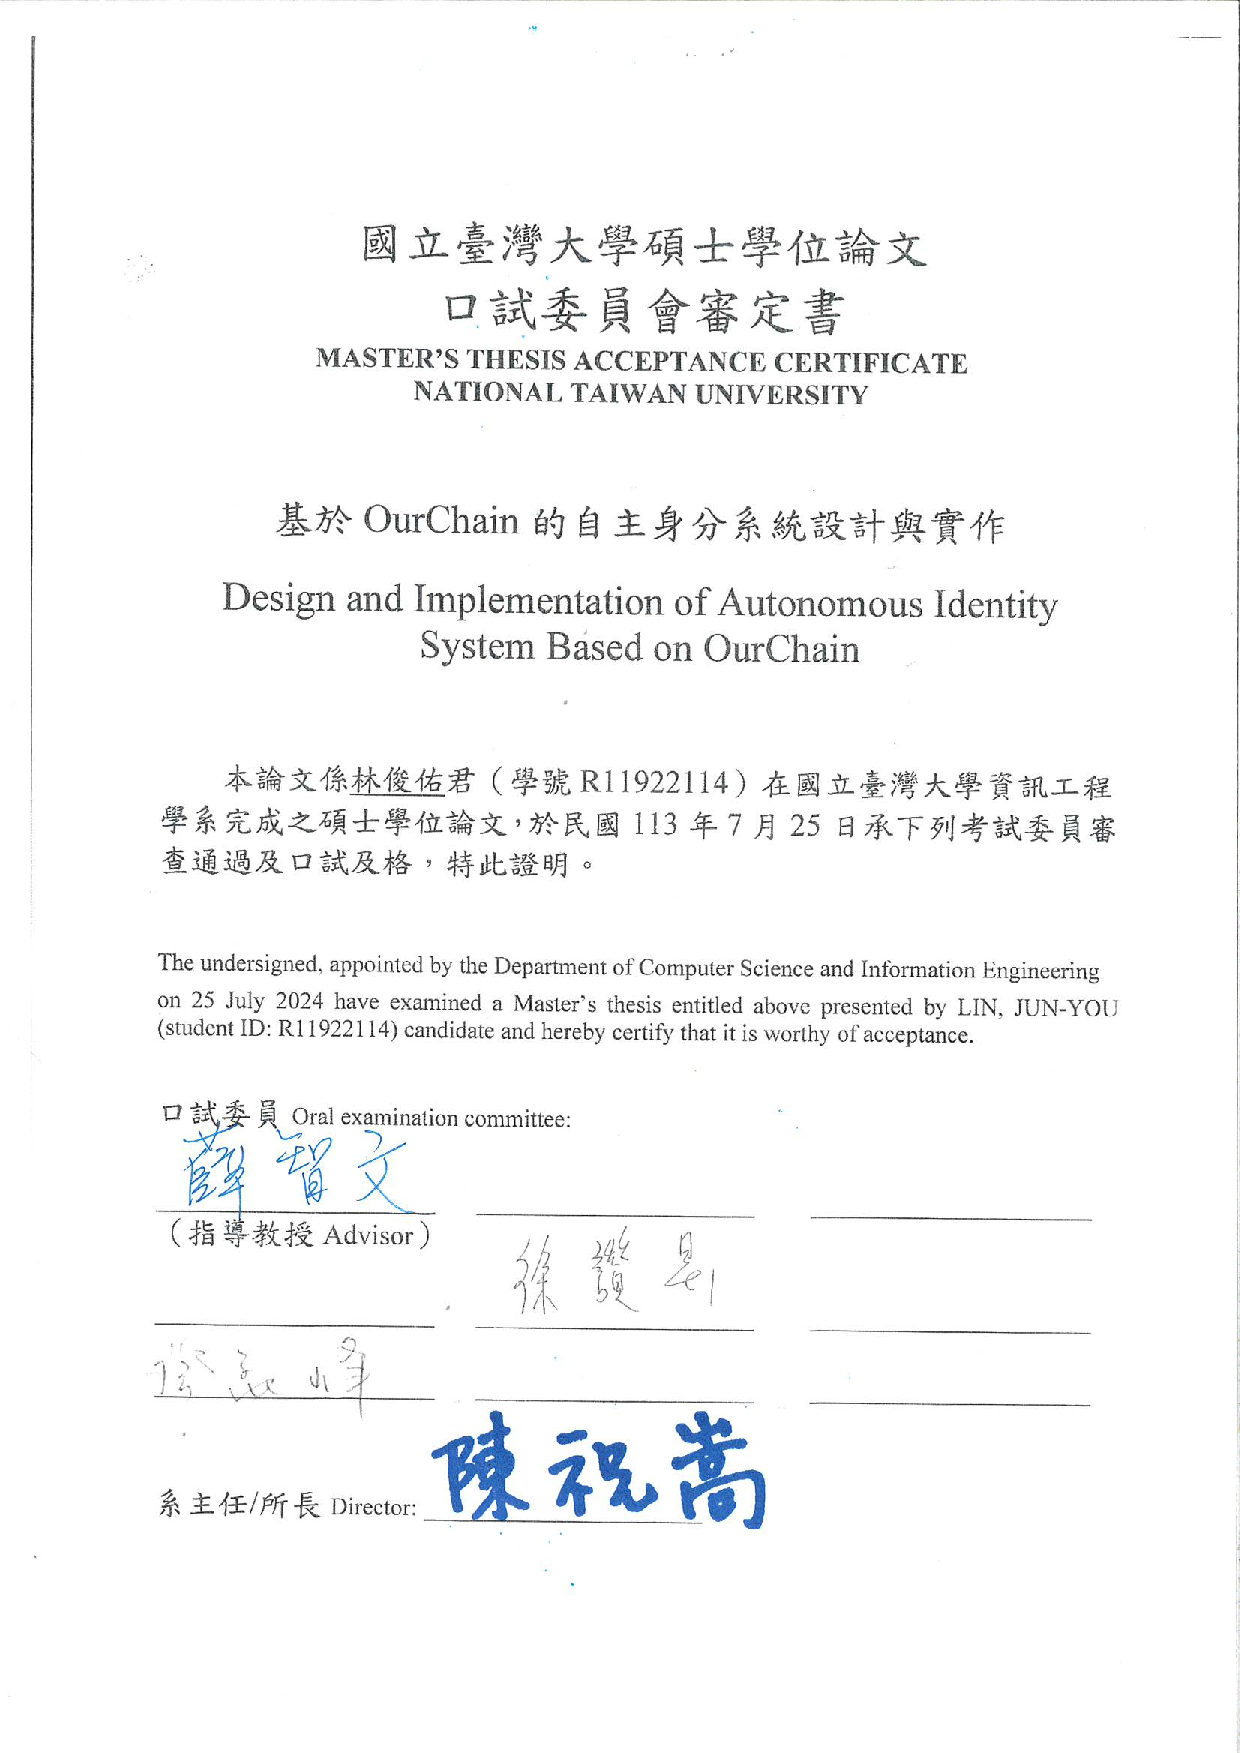
\includepdf[pages={1}]{docs/sign.pdf} % 真正口委簽名掃描

% 致謝與論文摘要
% Acknowledgement and Abstract
% !TeX root = ../main.tex

\begin{acknowledgement}

  致謝文打在這裡。致謝文打在這裡。致謝文打在這裡。致謝文打在這裡。致謝文打在這裡。致謝文打在這裡。致謝文打在這裡。致謝文打在這裡。致謝文打在這裡。致謝文打在這裡。致謝文打在這裡。致謝文打在這裡。致謝文打在這裡。致謝文打在這裡。致謝文打在這裡。致謝文打在這裡。致謝文打在這裡。致謝文打在這裡。致謝文打在這裡。致謝文打在這裡。致謝文打在這裡。致謝文打在這裡。致謝文打在這裡。致謝文打在這裡。致謝文打在這裡。致謝文打在這裡。致謝文打在這裡。致謝文打在這裡。致謝文打在這裡。致謝文打在這裡。致謝文打在這裡。致謝文打在這裡。致謝文打在這裡。致謝文打在這裡。致謝文打在這裡。致謝文打在這裡。致謝文打在這裡。致謝文打在這裡。致謝文打在這裡。致謝文打在這裡。致謝文打在這裡。致謝文打在這裡。致謝文打在這裡。致謝文打在這裡。致謝文打在這裡。致謝文打在這裡。致謝文打在這裡。

\end{acknowledgement}       % 致謝(Acknowledgement)
% !TeX root = ../main.tex

\begin{abstract}
  現代數位身分系統面臨嚴峻挑戰:身分驗證漏洞威脅用戶安全,中央化數據儲存易遭攻擊導致大規模個資外洩,大型組織壟斷關鍵服務造成權力失衡。這些問題不僅危及個人權益,更阻礙了數位社會的發展。本研究將完善「自主身分」系統,旨在徹底重塑數位身分管理。本研究從身分認證、資料管理和信用評分三個關鍵領域著手,設計了一套去中心化解決方案,成功將數位身分的控制權從大型機構手中歸還給個人用戶,顯著提升了用戶自主權。本研究還基於區塊鏈OurChain進行了概念驗證,成功證實了AID系統的可行性。本研究認為「自主身分」系統有潛力徹底改變人們與數位世界的互動方式,為建立一個更安全、公平和自由的數位社會鋪平道路。
\end{abstract}

\begin{abstract*}
  The modern identity systems have confronted with serious challenges: authentication vulnerabilities threaten user security, centralized data storage is vulnerable to large-scale data breaches, and core services monopolized by large organizations bring about power imbalance. These issues not only endanger individual rights but also hinder the development of digital society. This research aims to improve the "Autonomous Identity" system, with the goal of fundamentally reshaping digital identity management. Focusing on three crucial areas: identity authentication, data management, and credit scoring. We design a decentralized solution that returns the control of digital identity from large institutions to individual users, significantly enhancing user autonomy. We also conducted a proof of concept based on the OurChain, successfully demonstrating the feasibility of the AID system. This study believes that the "Autonomous Identity" system has the potential to completely change the way people interact with the digital world, paving the way for a safer, fairer, and freer digital society.
\end{abstract*}              % 摘要(Abstract)

% 生成目錄與符號列表
% Contents of Tables and Denotation
\maketableofcontents                % 目錄(Table of Contents)
\makelistoffigures                  % 圖目錄(List of Figures)
\makelistoftables                   % 表目錄(List of Tables)

% 論文內容
% Contents of Thesis
\mainmatter
% !TeX root = ../main.tex

\chapter{緒論}
在當今數位時代,個人身分管理已成為一個日益重要且複雜的議題。隨著網絡技術的快速發展和社會對隱私保護的日益重視,傳統的身分管理系統面臨著前所未有的挑戰。本研究旨在探討一種創新的解決方案——自主身分(Autonomous Identity,AID)系統,該系統融合了新的思想與先進技術,為數位身分管理帶來根本性的變革。通過重新審視「自主」的概念並將其應用於身分管理領域,我們希望能夠為構建一個更自由、更公平的數位社會貢獻一份力量。
\section{研究背景}
自主(Autonomy)概念源於18世紀啟蒙運動,標誌著人類開始質疑對王權與神權的依賴,轉而追求通過科學與理性實現思想獨立與自由。啟蒙思想家伊曼努爾·康德(Immanuel Kant)對自主提出了開創性定義:「按照自己認同的道德標準自由行事」。這一定義至今仍廣泛被應用於政治、法律和教育等多個領域。接著,19世紀的重要哲學家弗里德里希·尼采(Friedrich Nietzsche)對道德提出了更深入的探討。他對道德的本質進行了批判性分析,認為道德源於弱者對強者的反抗,是一種透過集結群體的共識來約束個體行為的機制。

這兩位哲學家的思想不僅塑造了現代社會對自主的理解,也為我們重新思考數位時代的身分管理提供了重要的理論基礎。隨著網絡技術的飛速發展,個人身分資訊的管理與保護已成為當今社會的重要議題。在這一背景下,我們將自主的概念創新性地應用於數位身分管理領域。

本研究提出的「自主身分」(Autonomous Identity,AID)概念與目前主流探討的「自治身分」(Self-sovereign identity,SSI)系統有著本質的區別。SSI允許使用者參與身分管理系統的經營,賦予使用者對其數位身分的一定控制權。然而,AID則更進一步,使每位使用者在具備\textbf{道德標準}的身分系統中\textbf{自由的管理自己}。這種創新模式不僅賦予使用者更大的自主權,還在系統設計中納入了道德考量,以確保個人自主不會損害社會整體利益。
\section{研究目的與目標}
本研究旨在探討自主身分(Autonomous Identity,AID)作為解決當前身分管理問題的創新方案,並將「自主」的哲學思想融入數位身分管理的實踐中。具體而言,本研究將致力於實現以下目標:
\begin{enumerate}
  \item \textbf{分析現有數位身分系統的局限性}:深入探討當前身分管理系統的主要挑戰和固有限制。
  \item \textbf{構建AID系統的理論框架}:提出自主身分系統的核心理念,並闡述其如何解決現有系統的問題。
  \item \textbf{設計AID系統的技術架構}:提出一種能夠實現使用者完全自主管理的技術方案,包括去中心化存儲、智能合約等關鍵技術的應用。
  \item \textbf{評估AID系統的優勢與挑戰}:全面比較AID系統與傳統身分管理系統在多方面的差異,並分析AID系統在實際應用中可能面臨的挑戰。
  \item \textbf{提出AID系統的未來展望}:探討AID系統在不同領域(如金融、醫療、政務等)的潛在應用場景,並提出相應的實施策略和路線圖。
\end{enumerate}
最終,我們希望這項研究能夠推動數位身分管理領域的典範轉移,為構建更加安全、自由、便捷和公平的數位社會奠定基礎。
\section{論文架構}
為了基於自主的理念設計出一個完整的身分驗證系統,我們需要先了解現有的身分驗證技術,並且對於這些技術進行分析,找出其缺點(第二章)。接著提出我們的系統設計,並且說明其架構、資料結構與威脅模型(第三章)。最後,我們會透過實作來驗證我們的系統設計(第四章),最終我們會提出結論與對方案的未來展望(第五章)。
% !TeX root = ../main.tex

\chapter{文獻探討}
身分系統的發展經歷了從中心化到去中心化的演變,現代身分系統設計面臨著使用者體驗、認知負擔、隱私保護和平等信任等多方面的挑戰,需要同時滿足技術創新、法規遵循和行業最佳實踐,以創造出既能滿足多樣化需求又具備足夠靈活性的解決方案,本章將探討相關文獻以深入理解這些挑戰及可能的解決途徑。
\section{身分系統的想像}
網際網路(Internet)發源於20世紀70年代,逐漸發展成為現代網際網路的基礎架構。最初,Internet的設計源自美國國防部的ARPANET計畫,旨在滿足軍事需求下的網路可用性和穩定性。因此,其初期設計基於以下假設\cite{Pekka2010HIP}:
\begin{itemize}
  \item 最終使用者至少在最低程度上相互信任。
  \item 網路由於潛在的物理攻擊而本質上不可靠。
\end{itemize}
這些假設在當時的網路環境中是合理的。然而,隨著網路的普及和應用範圍的擴大,這些假設已不再適用\cite{tomorrowinternet}。隨著Internet從一個研究驅動的項目演變為主流社會的重要組成部分,新的需求不斷湧現,不僅挑戰了原有的設計原則,還促使我們重新審視一些既有的假設。

在現代網路環境中,使用者之間的信任關係變得日益複雜。人們需要可靠的方式來識別自己和他人,以便在網路上進行交流和交易。因此,各種身分系統應運而生,以滿足網路環境中的身分識別需求。儘管人們希望找到一種統一而理想的身分管理系統,但正如Cameron\cite{cameron2005laws}所指出的,這樣的系統實際上並不存在。身分系統涉及的範疇廣泛而複雜,個人與組織之間存在多樣化且往往相互衝突的需求,試圖通過單一標準來限制或規範這些需求是不切實際的。

例如,終端使用者可能希望自由地訪問和分享信息,而內容提供商和知識產權持有者則希望保護其知識產權。政府可能希望監管某些網絡活動以維護社會秩序,而使用者和隱私倡導者則強調個人隱私的重要性。這種複雜的利益衝突導致了諸如網絡中立性、數據隱私、內容審查等一系列熱點問題的出現\cite{Wu2003NetworkNeutrality}。

面對這種複雜的網絡環境,Blumenthal\cite{Blumenthal2001RethinkingThe}認為確保設計上的一般性、彈性與開放性至關重要。他設想的未來充滿衝突:企業的管理者和被管理者爭論分紅,垃圾郵件的發送者和接收者爭論各自的困難。在這個網路世界中,不同身分的參與者沒有絕對的贏家,也沒有天生的失敗者。理想的系統應該通過所有使用者不斷的爭論和互動逐漸形成。

這種新的設計思路不僅需要考慮技術因素,還需要權衡經濟、社會、法律等多方面的因素。正如Lessig\cite{lessig2000}所言,"程式碼就是法則"("Code is Law")。軟體設計本身就在表達某種價值觀,人們需要縝密的思考,結合對未來世界的想像,才能創造出足以改變網路環境既有困境的身分系統。

總的來說,現代網路環境的變遷對身分系統提出了新的挑戰,這些挑戰不僅來自技術層面,還涉及社會、文化和法律等多個方面。為了應對這些挑戰,我們需要重新思考身分系統的設計理念,尋找一種既能適應當前多樣化需求,又能為未來發展預留足夠靈活性的解決方案。
\section{身分系統的迭代}
身分系統的設計經歷了多個階段的演變,每個階段都試圖解決特定的問題,同時也帶來了新的挑戰。本節將介紹不同世代的身分系統設計,以說明彼此衝突的需求和技術限制,並為後續討論提供背景。
\subsection{中心化身分}
\begin{figure}
  \centering
  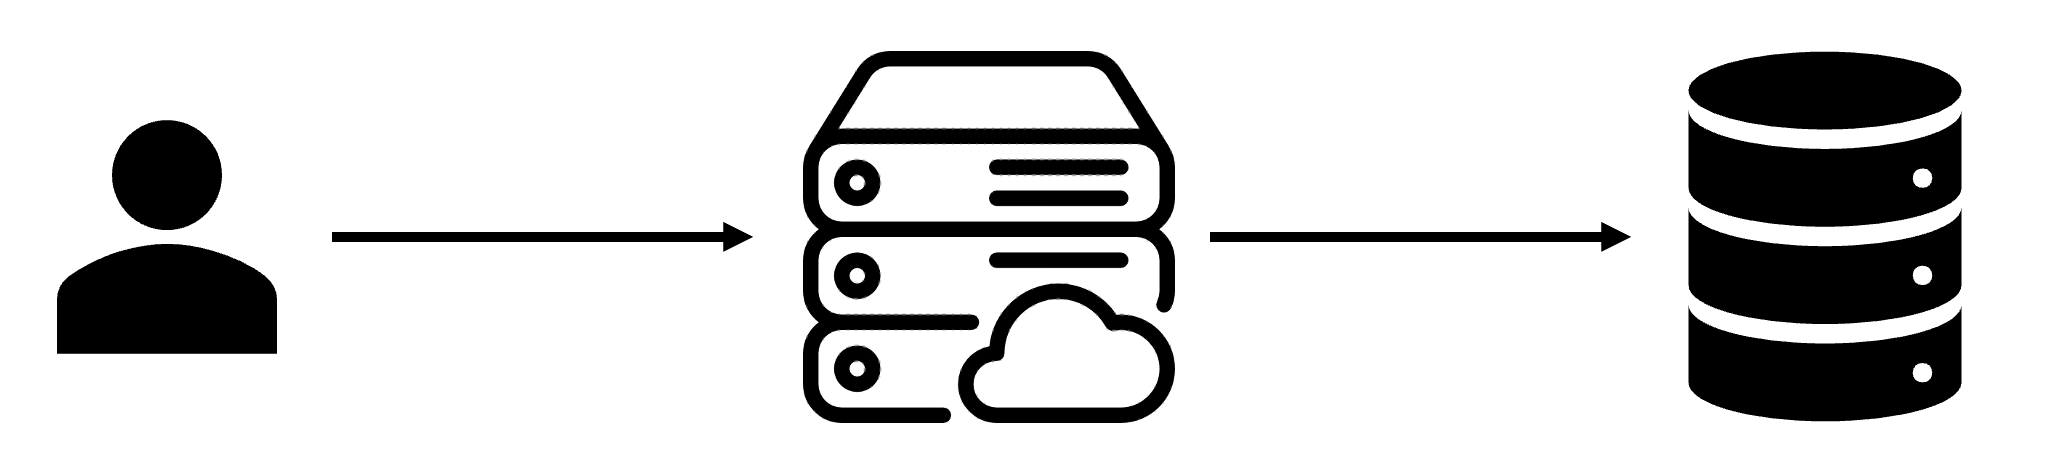
\includegraphics[width=\linewidth,keepaspectratio]{figures/mid-identity.png}
  \caption{中心化身分}
  \label{fig:mid-identity}
\end{figure}
中心化身分系統如圖\ref{fig:mid-identity}是最早期的身分管理方案,由同一位管理者操作和存儲所有使用者資訊,在企業和政府機構中廣泛應用。典型例子包括活動目錄(Windows Active Directory, AD)和輕量級目錄訪問協議(Lightweight Directory Access Protocol, LDAP)\cite{microsoft2021active, sermersheim2006lightweight}。這類系統的主要優勢在於其集中管理的特性,便於系統管理員進行使用者管理和權限控制,同時確保組織內部身分信息的一致性和及時更新。然而,中心化身分系統也面臨著諸多挑戰,如單點故障風險、隱私保護問題,以及跨組織可遷移性差等。使用者通常需要為每個服務創建單獨帳戶,這不僅增加了認知負擔\cite{josang2007security},還導致使用者身分被服務提供商完全控制,缺乏自主權。
\subsection{聯合身分}
\begin{figure}
  \centering
  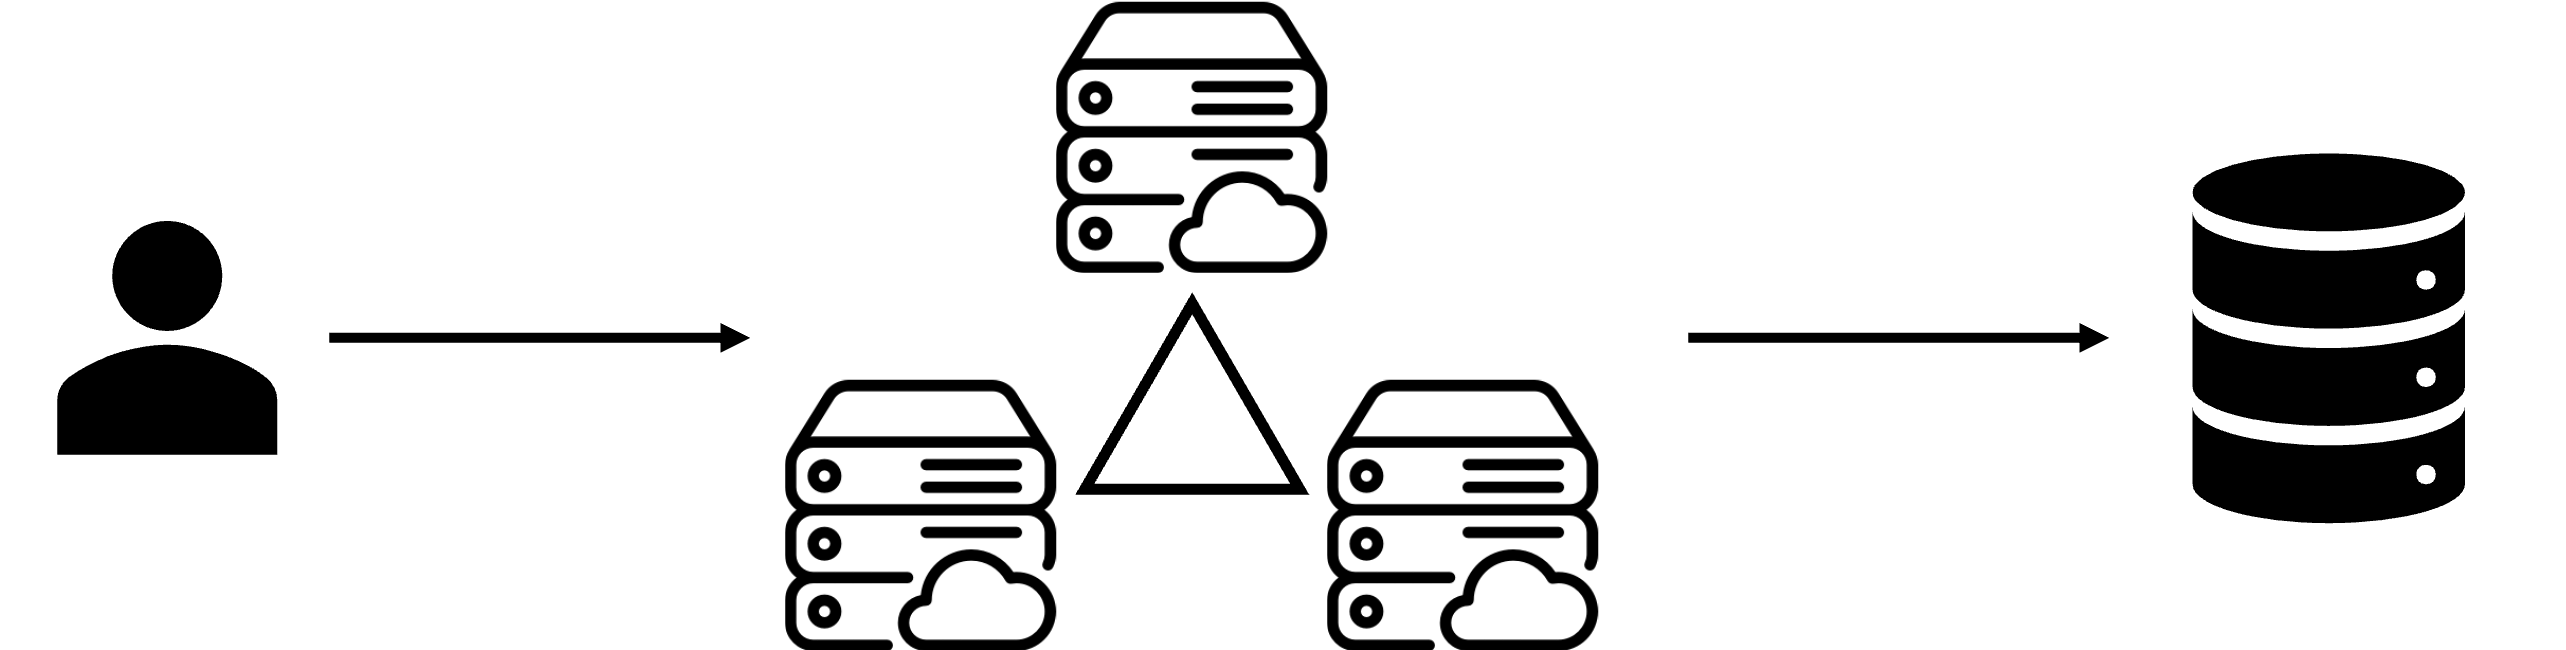
\includegraphics[width=\linewidth,keepaspectratio]{figures/group-identity.png}
  \caption{聯合身分}
  \label{fig:group-identity}
\end{figure}
主要為了解決同一個使用者擁有太多身分的認知負擔,聯合身分系統如圖\ref{fig:group-identity}允許不同組織間共享身分信息,代表性技術包括安全斷言標記語言(Security Assertion Markup Language, SAML)和 WS-Federation \cite{oasis2005security, goodner2009web}。這種模式的出現大大改善了使用者體驗,實現了單點登錄(Single sign-on,SSO),減少了密碼疲勞問題。聯合身分系統促進了組織間的協作和資源共享,同時也降低了重複身分管理的運營成本。然而,這種模式也帶來了隱私方面的挑戰\cite{ahn2007user},如使用者信息在多個服務提供商間共享可能違反《通用資料保護規則》(General Data Protection Regulation,GDPR)\cite{GDPR2016}等隱私法規。此外,實施和維護聯合身分系統的技術複雜度較高,參與組織之間需要建立並維護信任關係。\newpage
\subsection{使用者中心的身分}
\begin{figure}
  \centering
  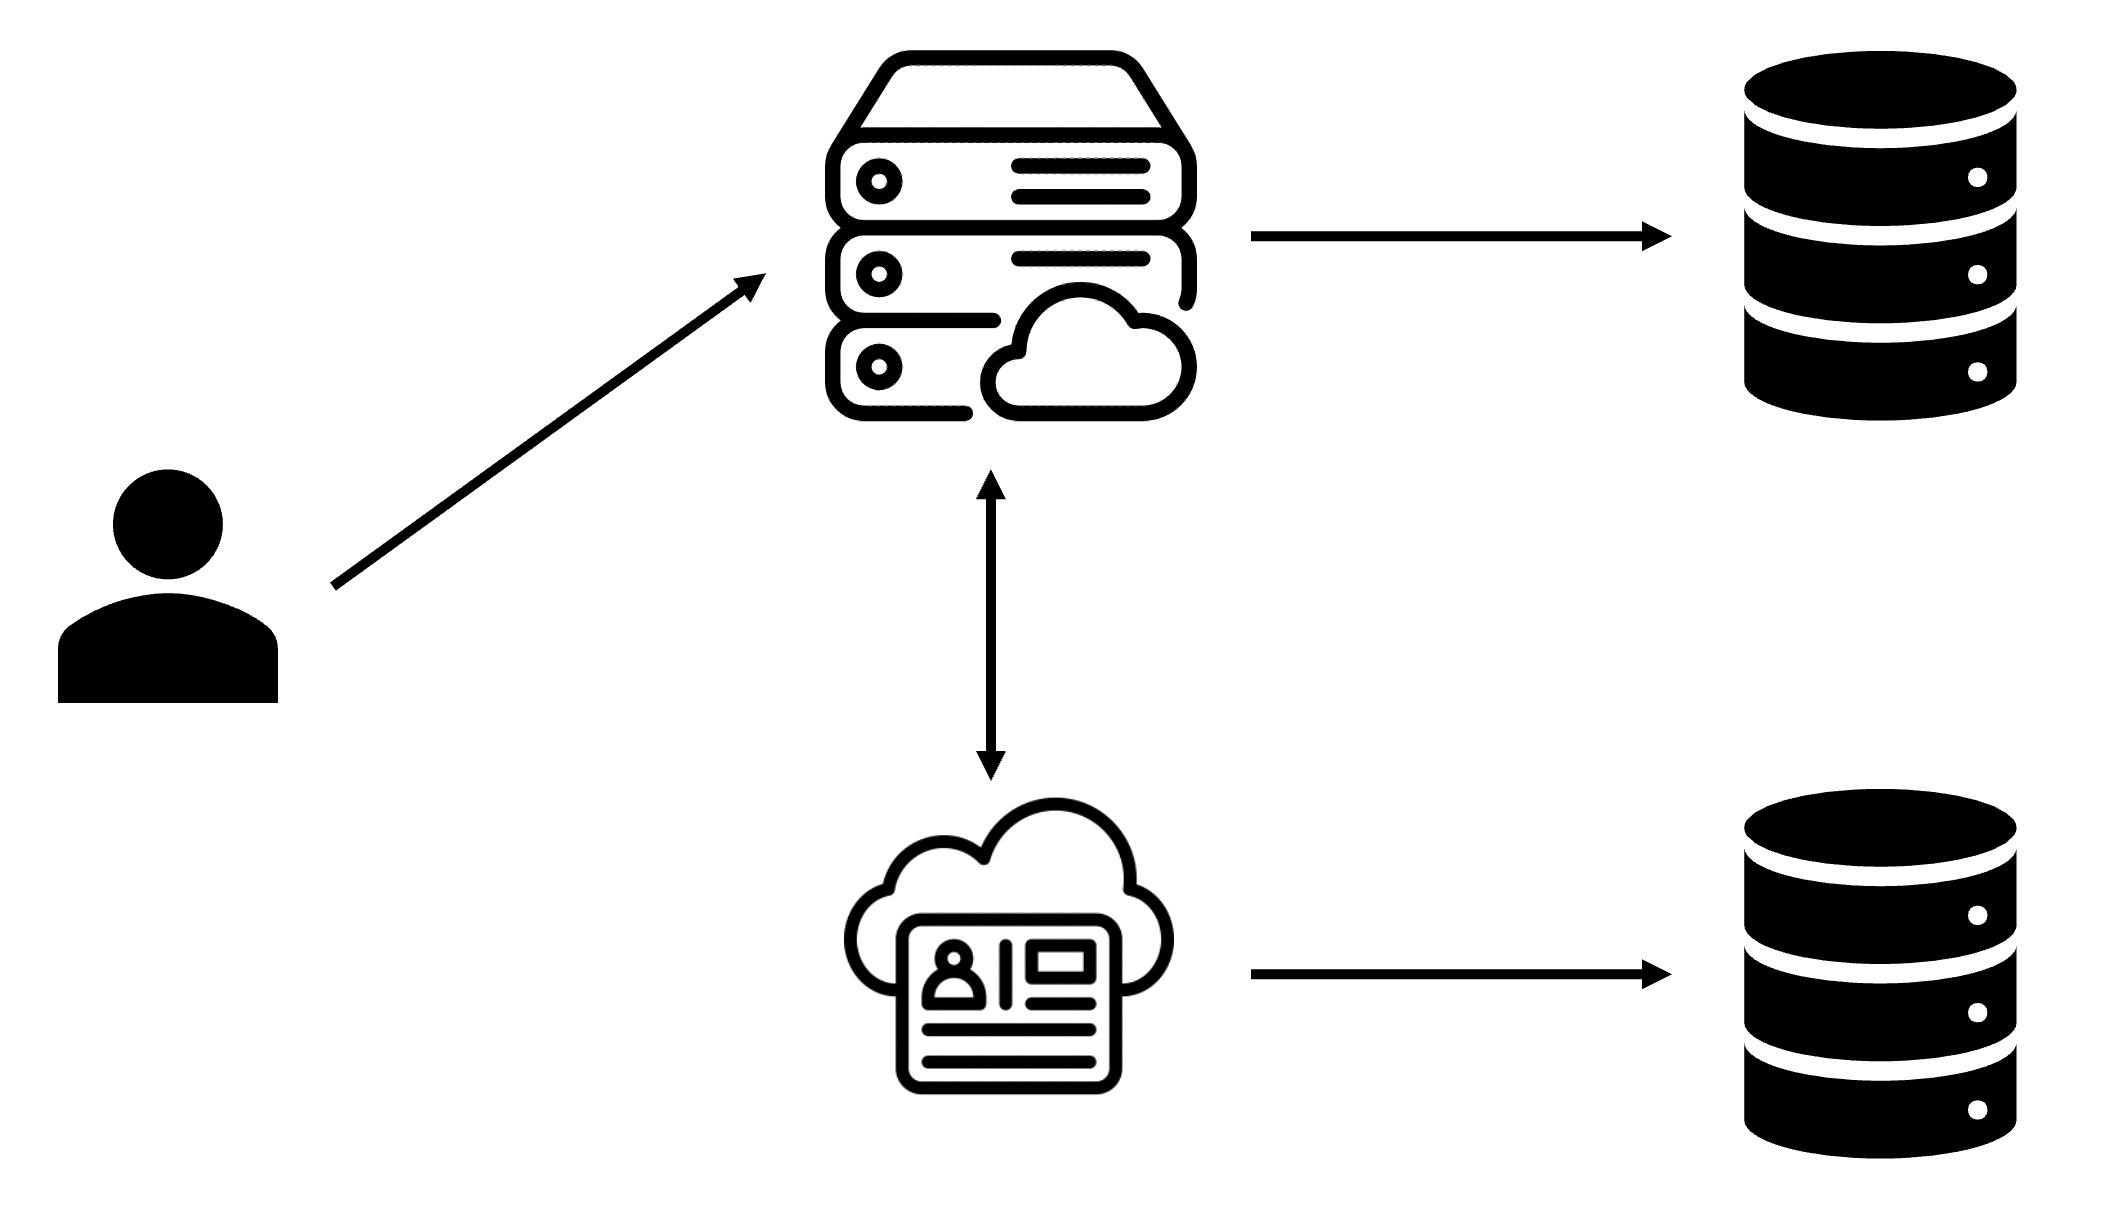
\includegraphics[width=\linewidth,keepaspectratio]{figures/user-mid-identity.png}
  \caption{使用者中心身分}
  \label{fig:user-mid-identity}
\end{figure}
為了解決隱私方面的問題,使用者中心的身分系統如圖\ref{fig:user-mid-identity}所示逐漸興起。這種系統允許使用者透過單一的身分供應者登入多個獨立的服務,同時每個服務各自掌握使用者在其內部的資料。隨著這種需求的增長,新的技術標準應運而生。OpenID和OAuth等協議的出現\cite{sakimura2014openid, hardt2012oauth},標誌著身分管理向使用者賦權的重要轉變。這種模式增強了使用者對個人身分信息的控制權,提供了更大的靈活性,允許使用者選擇不同的身分提供者。

使用者中心的身分系統實現了以服務供應商為單位的資訊範圍控制,在一定程度上改善了隱私保護。然而,這種方式也面臨著一些挑戰。首先是身分碎片化的問題,多個身分提供者的存在可能導致使用者體驗的不一致。其次,安全風險如釣魚攻擊和身分提供者數據洩露等仍然存在\cite{sun2012devil}。此外,儘管使用者獲得了更多控制權,但他們仍然在某種程度上依賴中心化的身分提供者,因此使用者的自主性還擁有很大的提升空間\cite{allen2016selfsovereign}。
\subsection{自治身分}
\begin{figure}
  \centering
  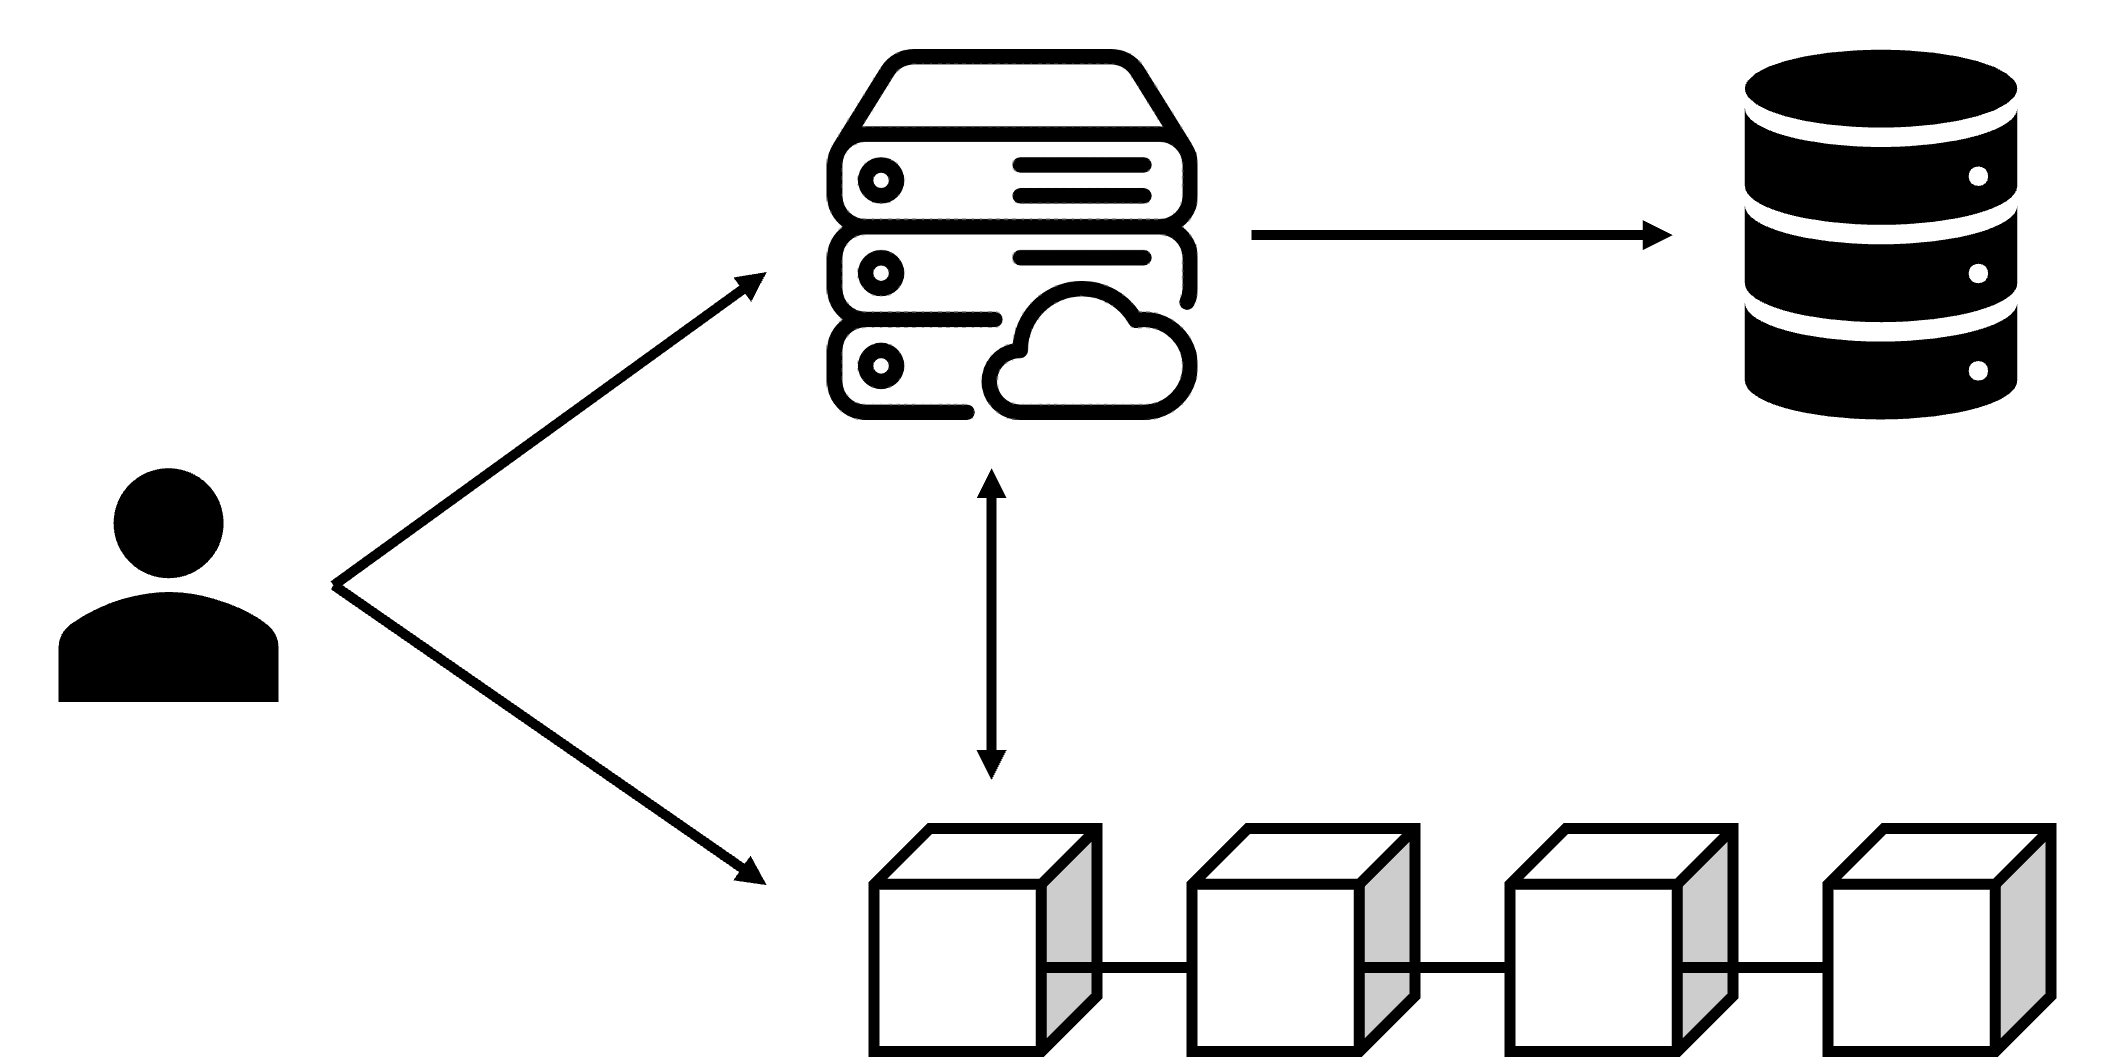
\includegraphics[width=\linewidth,keepaspectratio]{figures/self-sovereign-identity.png}
  \caption{自治身分}
  \label{fig:self-sovereign-identity}
\end{figure}
自治身分如圖\ref{fig:self-sovereign-identity}所示,是身分管理系統的最新發展\cite{preukschat2021self}。這種方式透過區塊鏈技術取代中心化的身分供應商,其代表性例子包括基於以太坊的uPort和微軟的自治身分覆蓋網絡\cite{lundkvist2017uport, microsoft2020ion}。自治身分系統賦予使用者對自身身分的控制權與對身分管理的治理權,同時提高了身分的可攜性和一致性。此外,它還增強了使用者與服務提供商之間的平等性,並提供了抗審查的特性。

然而,作為一種新興技術,自治身分系統也面臨著諸多挑戰\cite{s22155641}:
\begin{itemize}
  \item \textbf{法律框架衝突:} 它可能與現有法律框架存在潛在衝突,例如與GDPR中的被遺忘權不相容\cite{finck2018blockchains}。
  \item \textbf{技術複雜性:} 自治身分系統的技術複雜性可能影響普通使用者的使用體驗,降低其易用性\cite{kubach2020self}。
  \item \textbf{其他問題:} 還有諸如隱私保護、系統互操作性等問題需要解決。
\end{itemize}
\subsection{未來展望}
綜上所述,身分系統的發展經歷了多個階段,每個階段都試圖解決特定的問題。從中心化到使用者自治,身分系統的設計逐漸向使用者賦權,提高了使用者對自身身分的控制權。然而,即使到了使用者自治階段,我們依舊不認為找到了理想的解決方案。如同Schardong等人\cite{s22155641,soltani2021surveydid}所說,當今的自治身分系統仍面臨著許多挑戰,包括安全性、隱私保護、易用性、信任建立等問題。因此,我們認為身分系統的設計仍有很大的改進空間,需要更多的研究和實踐來不斷優化。
\section{身分系統的困境}
為了設計出一個理想的身分系統,在本節中,我們會從不同維度的多個方向來探討身分系統的困境。這些討論旨在幫助我們理解身分系統的核心特徵,並為未來的設計提供參考。
\subsection{使用者體驗}
使用者體驗在身分系統設計中扮演著關鍵角色,直接影響系統的可用性和採納率。然而,Hamme等人\cite{inproceedings}的研究闡明了使用者體驗、安全性和隱私保護之間的複雜關係。該研究指出了一個普遍存在的現象:使用者傾向於選擇最簡單的方式來設置和使用身分系統,這種傾向可能導致系統安全性和隱私保護程度的降低。

這種情況產生了一個兩難困境,為了提高安全性而強制使用者採用複雜的身分驗證方式可能會適得其反。例如Zhang等人\cite{zhang2010security}的研究表明,要求使用者定期更改密碼往往導致使用者僅修改特定字元,反而造成更大的安全隱患。同樣地,為了增強隱私保護而要求使用者完成詳細的隱私設置也可能降低使用者體驗。Acquisti等人\cite{acquisti2017nudges}的研究發現,複雜的隱私設置過程往往讓使用者感到困惑和沮喪,甚至導致他們放棄設置而選擇默認選項,從而降低了隱私保護水平。

為解決這一困境,研究者提出了「無摩擦驗證」(Zero Friction Authentication)的概念,旨在最小化使用者在設置和使用過程中遇到的困難,同時維持適當的安全性和隱私保護水平。Hamme等人\cite{inproceedings}強調,無摩擦驗證的核心目標是在保護使用者安全和隱私的同時,顯著降低使用者的操作負擔。這種平衡對於現代身分系統的設計至關重要,因為它直接影響系統的使用率和效能。

為實現無摩擦驗證,近年來安全領域出現了多種新技術。如Ghorbani等人\cite{ghorbani2020fido2}研究了無密碼登入(如FIDO2)的可用性,發現這種方法能透過硬體密鑰在手機上跨裝置完成高安全性的驗證,且使用者普遍認為方便並願意持續使用。Wiefling等人\cite{wiefling2021rba}探討了基於風險的驗證(Risk-Based Authentication,RBA),該方法透過追蹤身分與系統互動的歷史數據,在每次服務請求時動態判斷危險性,並在危險時採用更安全的多因素驗證(Multi-Factor Authentication,MFA)\cite{bonneau2012mfa}。Alaca等人\cite{alaca2016devicefingerprinting}關於裝置指紋的研究顯示,透過在每次使用者對服務發出請求時記錄並比對裝置指紋,可以有效辨識部分惡意行為,且不會增加使用者的操作負擔。

另外,為解決複雜隱私設置帶來的問題,Acquisti等人\cite{acquisti2017nudges}提出了「隱私設計」(Privacy by Design)的概念。這種方法將複雜的設置過程分解為多個簡單步驟,並在使用者使用系統的不同階段逐步引導使用者完成設置。研究表明,這種方法不僅能提高使用者的隱私保護水平,還能顯著改善使用者體驗。

這些新技術的應用表明,在不影響使用者體驗的前提下提供更高的安全性和更好的隱私保護是可能的。然而,如何在自主身分系統中實現真正的無摩擦驗證,以及如何有效地平衡使用者體驗、安全性和隱私保護的需求,仍然是一個值得深入研究的課題。
\subsection{使用者認知}
使用者認知在數位身分管理中扮演著至關重要的角色,直接影響到系統的安全性和有效性。LastPass\cite{lastpass2020psychology}的研究揭示了使用者認知與實際情況之間存在顯著差距:使用者平均估計自己擁有20個線上帳號,而實際上平均擁有37個以上的帳號。這種認知偏差背後反映了使用者使用上的不便,例如經常因為忘記密碼而無法登入帳號,或者因為各個帳號資料不互通而需要耗費大量時間來管理。

Dhamija等人\cite{dhamija2008sevenflaws}的研究進一步指出,使用者對身分管理系統的認知和理解程度直接影響其安全行為。隨著需要管理的使用者名和密碼數量增加,使用者往往感到困惑,進而採取不安全的行為,如使用弱密碼或在多個平台使用相同密碼等。此外,使用者對身分管理系統的認知不足也會導致他們無法有效應對釣魚攻擊、社交工程等安全威脅。

為了解決這個問題,未來的身分管理解決方案應該朝多個方向發展。首要任務是簡化多層次、多維度的使用者身分管理,允許單一的身分管理多樣的別名,以適用於不同的場景。例如,使用者可以用唯一的帳戶創建三個別名,分別對應自己的三種社會身分:在家中是家長,在工作中是員工,在社交場合是朋友。甚至針對單一的服務,使用者也可以擁有多種別名,如在論壇中既可以以專家身分發表權威言論,也可以作為普通使用者表達個人觀點。這樣的設計可以幫助使用者在盡可能不增加認知負擔的情況下有效管理自己的身分。

然而,真正簡化使用者認知並非易事。即使是宣稱已解決這個問題的使用者中心身分系統,實際上也未能完全做到。以Google的組織管理文件\cite{gcp2024identity}為例,為了確保不同組織擁有不同的安全限制與規定,系統仍然要求使用者在不同組織間創建不同的身分。這表明,同時簡化使用者認知與滿足組織需求,仍然是一個有待解決的挑戰。
\subsection{隱私保護}
在數位時代,隱私保護已成為身分系統設計的核心考量之一。歐盟制定的《通用數據保護條例》(GDPR)\cite{GDPR2016}代表了目前全球最嚴格的隱私保護標準。本研究認為,一個理想的身分系統應當能夠全面符合GDPR的要求,從而確保使用者隱私得到最大程度的保護。然而,近年來的GDPR違規案例表明,即便是大型企業也面臨著遵守某些GDPR規定的挑戰。

基於Schardong等人的研究\cite{s22155641},我們發現當前身分系統中存在兩個尤為突出的關鍵問題。首先是使用者積極授權的實現困難。Saemann\cite{saemann2022investigating}的研究強調,在當前的身分系統框架下,企業難以實現使用者對數據使用的明確授權。具體而言,企業難以證明其對數據或權限的使用行為已獲得使用者授權,而使用者也缺乏有效途徑證明自己的數據或權限被不當使用。這種情況不僅增加了企業的法律風險,也削弱了使用者對系統的信任。

第二個問題是被遺忘權的實現困難。Smirnova\cite{smirnova2024understanding}指出,滿足使用者的被遺忘權在當前身分系統中存在著一定的挑戰。使用者數據在系統中往往呈分散狀態,即使刪除核心使用者的資料,仍可能保留使用者的系統日誌或與其他使用者的互動數據。這種情況使得完全實現被遺忘權變得複雜而困難,可能導致使用者隱私無法得到全面保護。

基於以上分析,我們提出符合現代隱私保護要求的身分系統應該具備兩個關鍵特點。首先,系統應提供合理的機制,讓使用者或企業能夠證明其數據使用行為是否符合授權,這將有助於提高系統的透明度和可信度。其次,系統應提供有效的方法讓使用者行使被遺忘權,確保使用者不會被難以刪除的數據綁架。這意味著系統需要設計更精細的數據管理和刪除機制。在後續研究中,我們將詳細探討如何在自主身分系統中實現這些特性,並提出相應的技術解決方案。
\subsection{平等信任}
身分系統中的平等信任問題是一個複雜的多方利益平衡問題,涉及系統的公平性和可信度。研究\cite{preukschat2021self}強調了身分系統中各方利益的衝突,主要表現在使用者之間的權益差異、不同系統間的互操作性問題,以及使用者與系統供應者之間的利益衝突。例如,身分系統供應者可能希望獲取更多使用者個人資料以獲取利益,而使用者則希望保護自己的隱私。這種利益衝突如果處理不當,可能導致系統環境惡化、使用者權益受到侵犯,以及市場壟斷和不公平競爭。Zuboff\cite{zhang2010security}的研究進一步指出,這種數據收集和利用的不平等可能導致所謂的「監視資本主義」,對個人自由和社會公平造成深遠影響。

在當前的身分系統中,建立健全的信任模型仍然是一個重大挑戰。傳統的二元邏輯驗證模式(即完全信任或完全不信任)已不能滿足現代身分系統的需求。研究\cite{s22155641}指出,現實世界的信任往往是模糊而不確定的,人們很難用簡單的真假邏輯分辨使用者驗證的成功與否。例如,可能存在多組憑證同時存在,部分驗證成功,部分驗證失敗的情況,或者不同照照的可信度和重要性各不相同。Josang等人\cite{josang2006exploring}提出的主觀邏輯數學框架為處理這類多組不確定性證照的問題提供了一個系統性的解決方案。該框架將憑證的可信度表示為一個區間,從而更好地模擬了現實世界的身分驗證過程。

此外,在去中心化系統中,解決身分驗證問題尤其困難。正如Dhamija\cite{dhamija2008sevenflaws}所強調的,使用者需要向系統證明自己的身分,同時系統也需要向使用者證明自己的合法性和可信度。Tze-Nan\cite{NTU202102846}提出的自主證照機制為解決這一問題提供了一個新的思路。他改良了傳統的證照簽署(Certificate Authority)技術,使證照不僅可以由使用者自主操作,還能被所有經手者評分。這樣一來,使用者和系統之間就可以在自主的前提下互相驗證並評分,從而建立起一個平等的信任關係。

然而,長期來看,一個合理的評分機制,甚至是一個長期的治理機制也是必要的。在這方面,Chohan等人\cite{chohan2024decentralized}關於DAO(去中心化自治組織,Decentralized Autonomous Organization)治理的研究提供了核心概念,可以為自主身分系統的制度建設提供參考。

在後續的研究中,我們將探討如何在自主身分系統中實現技術上的互相驗證與制度上的互相信任,最終構建一個能夠平衡各方利益、促進公平競爭而不易壟斷的自主身分生態系統。這種系統將能夠在保護使用者權益的同時,也為系統供應者提供合理的發展空間,從而實現真正的平等信任。
\section{身分系統的評估}
鑒於當前身分系統在各個方面面臨的特定挑戰,我們提出以下評估標準,用以衡量自主身分系統的設計是否符合下一代身分系統的要求:
\begin{itemize}
  \item \textbf{創新突破}:自主身分系統的設計應解決上節所述困境,才能實現真正的技術創新。以下陳列:
        \begin{itemize}
          \item 使用者體驗:提供無摩擦驗證,簡化操作流程,提高系統易用性。
          \item 使用者認知:提供簡單的身分管理機制,幫助使用者有效管理身分,減少認知負擔。
          \item 隱私保護:實施有效的隱私保護機制,保護使用者個人數據,確保隱私得到充分保障。
          \item 平等信任:建立互相驗證和互相信任的機制,促進所有個體間平等的信任關係。
        \end{itemize}
  \item \textbf{法規遵循}:自主身分系統應符合相關法律法規,特別是在數據保護和隱私保護方面。例如:
        \begin{itemize}
          \item GDPR:遵守一般資料保護規範\cite{GDPR2016}的要求,包括使用者同意、數據可控性和被遺忘權等規定。
          \item NIST:符合美國國家標準\cite{NIST800-63-3},涵蓋多因素驗證、風險評估、身分驗證和授權等要求。
        \end{itemize}
  \item \textbf{公認原則}:遵循身分識別領域的公認原則,包括但不限於:
        \begin{itemize}
          \item 身分法則:符合Kim Cameron提出的身分管理基本法則\cite{cameron2005laws},包括使用者控制、最小化披露和互操作性等原則。
          \item 避免常見缺陷:克服Dhamija等人\cite{dhamija2008sevenflaws}指出的身分管理七大缺陷,如使用者體驗、使用者認知、使用者信任等問題。
          \item 自治身分:符合Allen\cite{allen2016selfsovereign}所說,自治身分應該遵循的10個原則。
        \end{itemize}
\end{itemize}
這些評估標準綜合考慮了技術創新、法律合規性和業界最佳實踐,為評估和設計下一代自主身分系統提供了全面的合理的目標。
\section{總結}
本章從身分系統的迭代、設計原則和技術評估三個方面探討了現代身分系統的設計問題。我們發現,現代身分系統的設計仍面臨著諸多挑戰,包括使用者體驗、使用者認知、隱私保護、平等信任等方面。為了解決這些問題,我們提出了一系列設計原則,包括無摩擦驗證、隱私設計、使用者認知簡化、......等。在未來的研究中,我們將進一步探討如何在自主身分系統中達到這些評估標準,並提出相應的技術解決方案。
% !TeX root = ../main.tex

\chapter{系統設計}
自主身份(AID)系統是一種創新的身份管理架構,其核心理念在於賦予個體對其身份資料的完全控制權。在這個系統中,三個關鍵角色相互協作:用戶、服務提供者和共識核心。用戶作為系統的終端使用者,通過個人設備全權管理自己的身份資料,根據需求選擇性地使用任意個服務並控制資料的流動。服務提供者則擔任用戶聚集的節點,不儲存用戶資料,而是根據用戶提供的資訊完成相應服務,並可靈活地根據實際場景客製化管理模式。共識核心則扮演著關鍵的中介角色,連接服務與服務、服務與用戶,提供用戶數據背書和信任評價機制,成為整個生態系統的基石。

本章節將深入探討此系統的架構設計、資料結構和潛在威脅模型,全面分析其如何在保障用戶自主權的同時,實現高效、安全的身份管理。
\section{系統的重要進步}
為實現用戶對其身份的完全自主權,本研究提出了多項創新機制,旨在解決現有的技術困境。
\subsection{別名優先機制}
傳統的身份驗證系統要求使用者提供唯一帳號作為登入識別。然而,這種設計無形中剝奪了用戶對個人名稱的自主權。一個連名稱都無法自主的系統,顯然難以達成本研究的設計目標。因此,我們提出讓用戶在註冊身份時優先使用自己喜歡的別名,再透過 UUID 機制\cite{uuid}作為唯一識別號。在日常操作中,系統優先讓用戶使用別名作為帳號,只有當別名因重複而難以識別時,才會要求用戶使用與 UUID 關聯的機制進行識別。當然,何時該使用別名,何時該使用 UUID,這是個複雜的問題。為此,我們提出了「基於用戶時空的分析方法」,試圖系統性地進行分析。
\subsection{基於用戶時空的分析方法}
每個身份本質上可視為一個隨時間變化的動態向量空間,其維度可謂無窮。每次對用戶的身份驗證都可視為取得特定時間僅含部分維度的向量。這方法的核心是讓用戶自主決定提供哪些維度,並在每次與系統互動時攜帶這些資訊。基於此概念,系統可藉由比對當次傳入的向量和近期暫存在快取中的所有向量來推測用戶的真實身份。

舉例來說:用戶在某次登入時提供了自己的別名、性別、所在地區等資訊,而在下次登入時僅提供了性別、所在地區等資訊,系統可以通過比對這兩次向量來推測用戶的別名。這種方法使用戶在不提供完整資訊的情況下,仍能通過部分資訊完成身份驗證。

然而,這種方法也帶來了一些問題。例如,用戶提供的維度多寡會影響系統的準確性,甚至用戶提供的維度是否包含可變資訊會影響系統的安全性。因此,我們提出維度的選擇甚至各個維度的權重應由用戶自主決定,而系統僅提供推薦機制。這樣可讓用戶在不同情境下使用不同方法,以滿足其需求。

總的來說,當僅有一個用戶被比較出來時視為可識別,有零個或多個用戶被比較出來時視為不可識別。這種機制受比較方法影響,因此我們提出了「基於危險程度的驗證機制」,希望能在不同情境下選擇適合的比較方法。
\subsection{基於危險程度的驗證機制}
此機制主要使用在比較身份與歷史紀錄時選擇適合的比較方法。不同的比較方法可能導致不同的結果,因其本質上代表了不同的嚴謹程度。在嚴謹程度較高的情況下,用戶可能需要更多維度符合,或需要在更接近的時間點內提供的紀錄才算數。這可能導致用戶難以找到識別對象,進而要求補充更多資訊再次驗證。相反,在嚴謹程度較低的情況下,用戶可能僅用少量維度的資訊配合較遠時間點的紀錄來完成驗證,這可能導致用戶被誤認為其他用戶,威脅系統安全。

考慮用戶行為的危險程度,我們設計出以下規則:
\begin{enumerate}
  \item 當用戶的行為被視為危險時,系統應提高驗證的嚴謹程度。
  \item 當用戶的行為被視為安全時,系統應降低驗證的嚴謹程度。
\end{enumerate}

接著,我們將嚴謹程度拆分為時間和空間兩個軸,使用笛卡爾座標系統表示,以細分出更複雜的情境:
\begin{enumerate}
  \item 當用戶行為超危險時,比較標準應為時間非常近或多個維度符合。
  \item 當用戶行為危險時,比較標準應為時間相對近或維度相對符合。
  \item 當用戶行為安全時,比較標準應為時間相對遠或維度相對不符合。
  \item 當用戶行為超安全時,比較標準應為時間非常遠或僅幾個維度符合。
\end{enumerate}

最後,用戶行為的危險程度在我們的系統中是由用戶自主決定的,系統僅提供推薦機制。我們希望藉此滿足所有用戶在各種情境下的需求。例如,對於個人銀行帳戶,可能所有行為都視為最高危險,因此需要最高的驗證嚴謹程度。而對於個人社群帳戶,讀取文章的行為可能視為不危險,發布文章則視為危險,因此需要不同的驗證嚴謹程度。我們建議用戶將危險的概念定義為對用戶數據變動的敏感程度:越敏感的數據越危險,越危險的數據越需要嚴謹的驗證機制。
\subsection{極致多因素認證}
傳統身份驗證系統中,多因素認證被廣泛使用,但僅被視為登入時的驗證方案。然而,我們認為多因素中的每個因素都可視為一個維度,而這些維度可由用戶自主選擇。因此,我們提出了極致多因素認證的概念:我們認為不存在特定的多因素驗證方法作為用戶登入的唯一方式,而應該反過來,從服務器的角度觀察,每個因素的驗證應該是用戶向服務器自主證明自己身份的方法。

因此,在足夠危險的情況下,可能需要連續多種因素的驗證;而在足夠安全的情況下,可能只需要一種因素的驗證。甚至即便遺失了某個重要因素,也不應被視為無法登入,而應被視為需要提供更多其他因素的驗證。
\subsection{自主證書}
本研究提出了一種創新的基於區塊鏈技術的自主身份驗證流程,旨在解決傳統身份管理系統中使用者對身份驗證缺乏自主權的問題。在傳統模式下,使用者的身份驗證資訊通常由身份服務提供者集中管理,這種做法實質上限制了使用者對其個人身份資訊的控制權。為了解決這一問題,我們參考了Tze-Nan\cite{NTU202102846}提出的自主證書機制,設計了一個基於區塊鏈技術的新型身份管理流程。

本研究提出的身份管理流程包含以下關鍵步驟:
\begin{enumerate}
  \item 簽章證書:使用者可以針對相同的自主身份在不同的簽章者處建立不同目的的證書,其內提供不同數據與權限。
  \item 區塊鏈驗證:證書的簽名會被簽章者記錄在區塊鏈上,服務提供者可以在區塊鏈上查詢證書的真實性,確保身份資訊的可信度。
  \item 證書撤銷:使用者可以隨時撤銷證書,並在區塊鏈上提交撤銷的簽名。這種機制可以應用於證書外流等情況,提高系統的安全性和可靠性。
  \item 自主註冊:使用者在註冊時,主動向服務提供者提交自己的證書,表明自己的身份。
  \item 彈性驗證:使用者在進行身份驗證時,可以根據證書自主選擇多因素驗證(MFA)的方式,提高身份驗證的便利性和安全性。
\end{enumerate}
此外,本系統的證書機制支援多樣化的功能,進一步提升了使用者對其身份資訊的控制權:
\begin{itemize}
  \item 自定義多因素認證選項
  \item 選擇性資訊揭露
  \item 設置證書有效期限
  \item 指定特定的驗證條件 (如特定設備,地點或時間)
  \item 指定特定的驗證規則(設備和網路使用限制)
  \item 資源存取權限控制 (如檔案存取權限)
\end{itemize}

總結來說,通過這種機制提升了系統對用戶隱私和安全的保護程度,讓用戶能夠更自主地管理其身份驗證流程,保持對個人身份驗證的控制權。
\subsection{數據共識}
在傳統身分管理系統中,基於安全和隱私的考慮,資料孤島問題一直難以有效解決。自主身分系統的出現為此提供了解決方案。使用者可以使用個人設備儲存自己的身份訊息,並在加入另一個自主身份系統時選擇性地上傳部分資訊。但這種設計仍然無法徹底解決資料孤島問題。尤其是當使用者想要共享的資料價值較高且可能被更改時,例如資產證明,此類資料無法僅在使用者的個人裝置上儲存和操作。

為了解決這一問題,本研究提出了一種基於區塊鏈的共識機制。在這種機制中,每個自主身份服務可以在區塊鏈上提交針對特定使用者特定數據的校驗簽名,進而讓其他服務能夠驗證使用者特定數據的真實性。這種設計使用戶能夠在不同的自主身份服務中安全地共享資料,同時向其他用戶保證資料的一致性和可信度。

這種基於區塊鏈的共識機制不僅有效解決了數據孤島問題,還提供了多方面的優勢。首先,通過區塊鏈技術確保了數據的完整性,有效防止數據被篡改。其次,它實現了使用者在不同自主身份系統間的無縫數據共享。再者,這種機制仍然保護了使用者的隱私,讓使用者能夠控制哪些數據被共享,保持對個人資訊的自主權。最後,它還支援實時驗證,其他服務可以即時驗證使用者數據的真實性,無需複雜的跨系統認證流程。
\subsection{自主身份數據管理}
基於前文所述的「自主證書機制」與「數據共識機制」,我們發展出了「自主身份數據管理」方法,旨在徹底解決被遺忘權和積極數據授權等棘手的隱私問題。在自主身份框架下,用戶通過自有裝置保存個人數據,包括證書與資料。當用戶需要證明身份時,需依照「自主證書機制」上傳證書給服務提供者,以完成對用戶的信任與驗證。而當用戶需要使用數據時,則上傳本地的相關數據,並可透過「數據共識機制」使服務提供者信任用戶所提供數據的真實性。

此外,針對特殊的隱私問題,自主身份數據管理提供了以下解決方案:
\begin{itemize}
  \item \textbf{被遺忘權}:當用戶希望遺忘數據時,可直接清除個人保留的數據。區塊鏈中僅保留簽名,而不保留數據本身。理論上,服務內部不會存儲用戶數據;即使確實存儲了,由於唯一能證明數據擁有人的是用戶本身,因此相當於用戶與數據無關。這個概念類似於 Cameron\cite{cameron2005laws}所描述的單向身份:用戶可以通過個人證明指向自己的數據,但僅有數據無法指向用戶。
  \item \textbf{積極數據授權}:採用類似「自主證書」的方法,使用戶與服務提供者對數據授權產生明確共識。當用戶授權服務提供者使用數據時,會對數據與使用範圍生成證書,並上傳對應簽名至區塊鏈,然後將證書與數據傳送給服務提供者。之後,用戶可利用公開證書證明數據被濫用,反之,服務提供者也可利用公開證書證明數據被合法使用。這樣的設計使用戶與服務提供者之間的數據授權變得更加明確且公平。
\end{itemize}

總的來說,自主身份數據管理方法提供了一個數據管理方法,讓用戶能夠更好地控制自己的數據,保護自己的隱私,並讓他人信任數據的真實性。\newpage
\section{系統架構}
自主身份系統如圖\ref{fig:aid-layers}所示,從宏觀來看可以被分成三個層次:由上而下分別是共識層、服務層與數據層。共識層負責確保數據的共識,服務層負責提供各種服務,數據層負責存儲用戶數據。
\begin{figure}
  \centering
  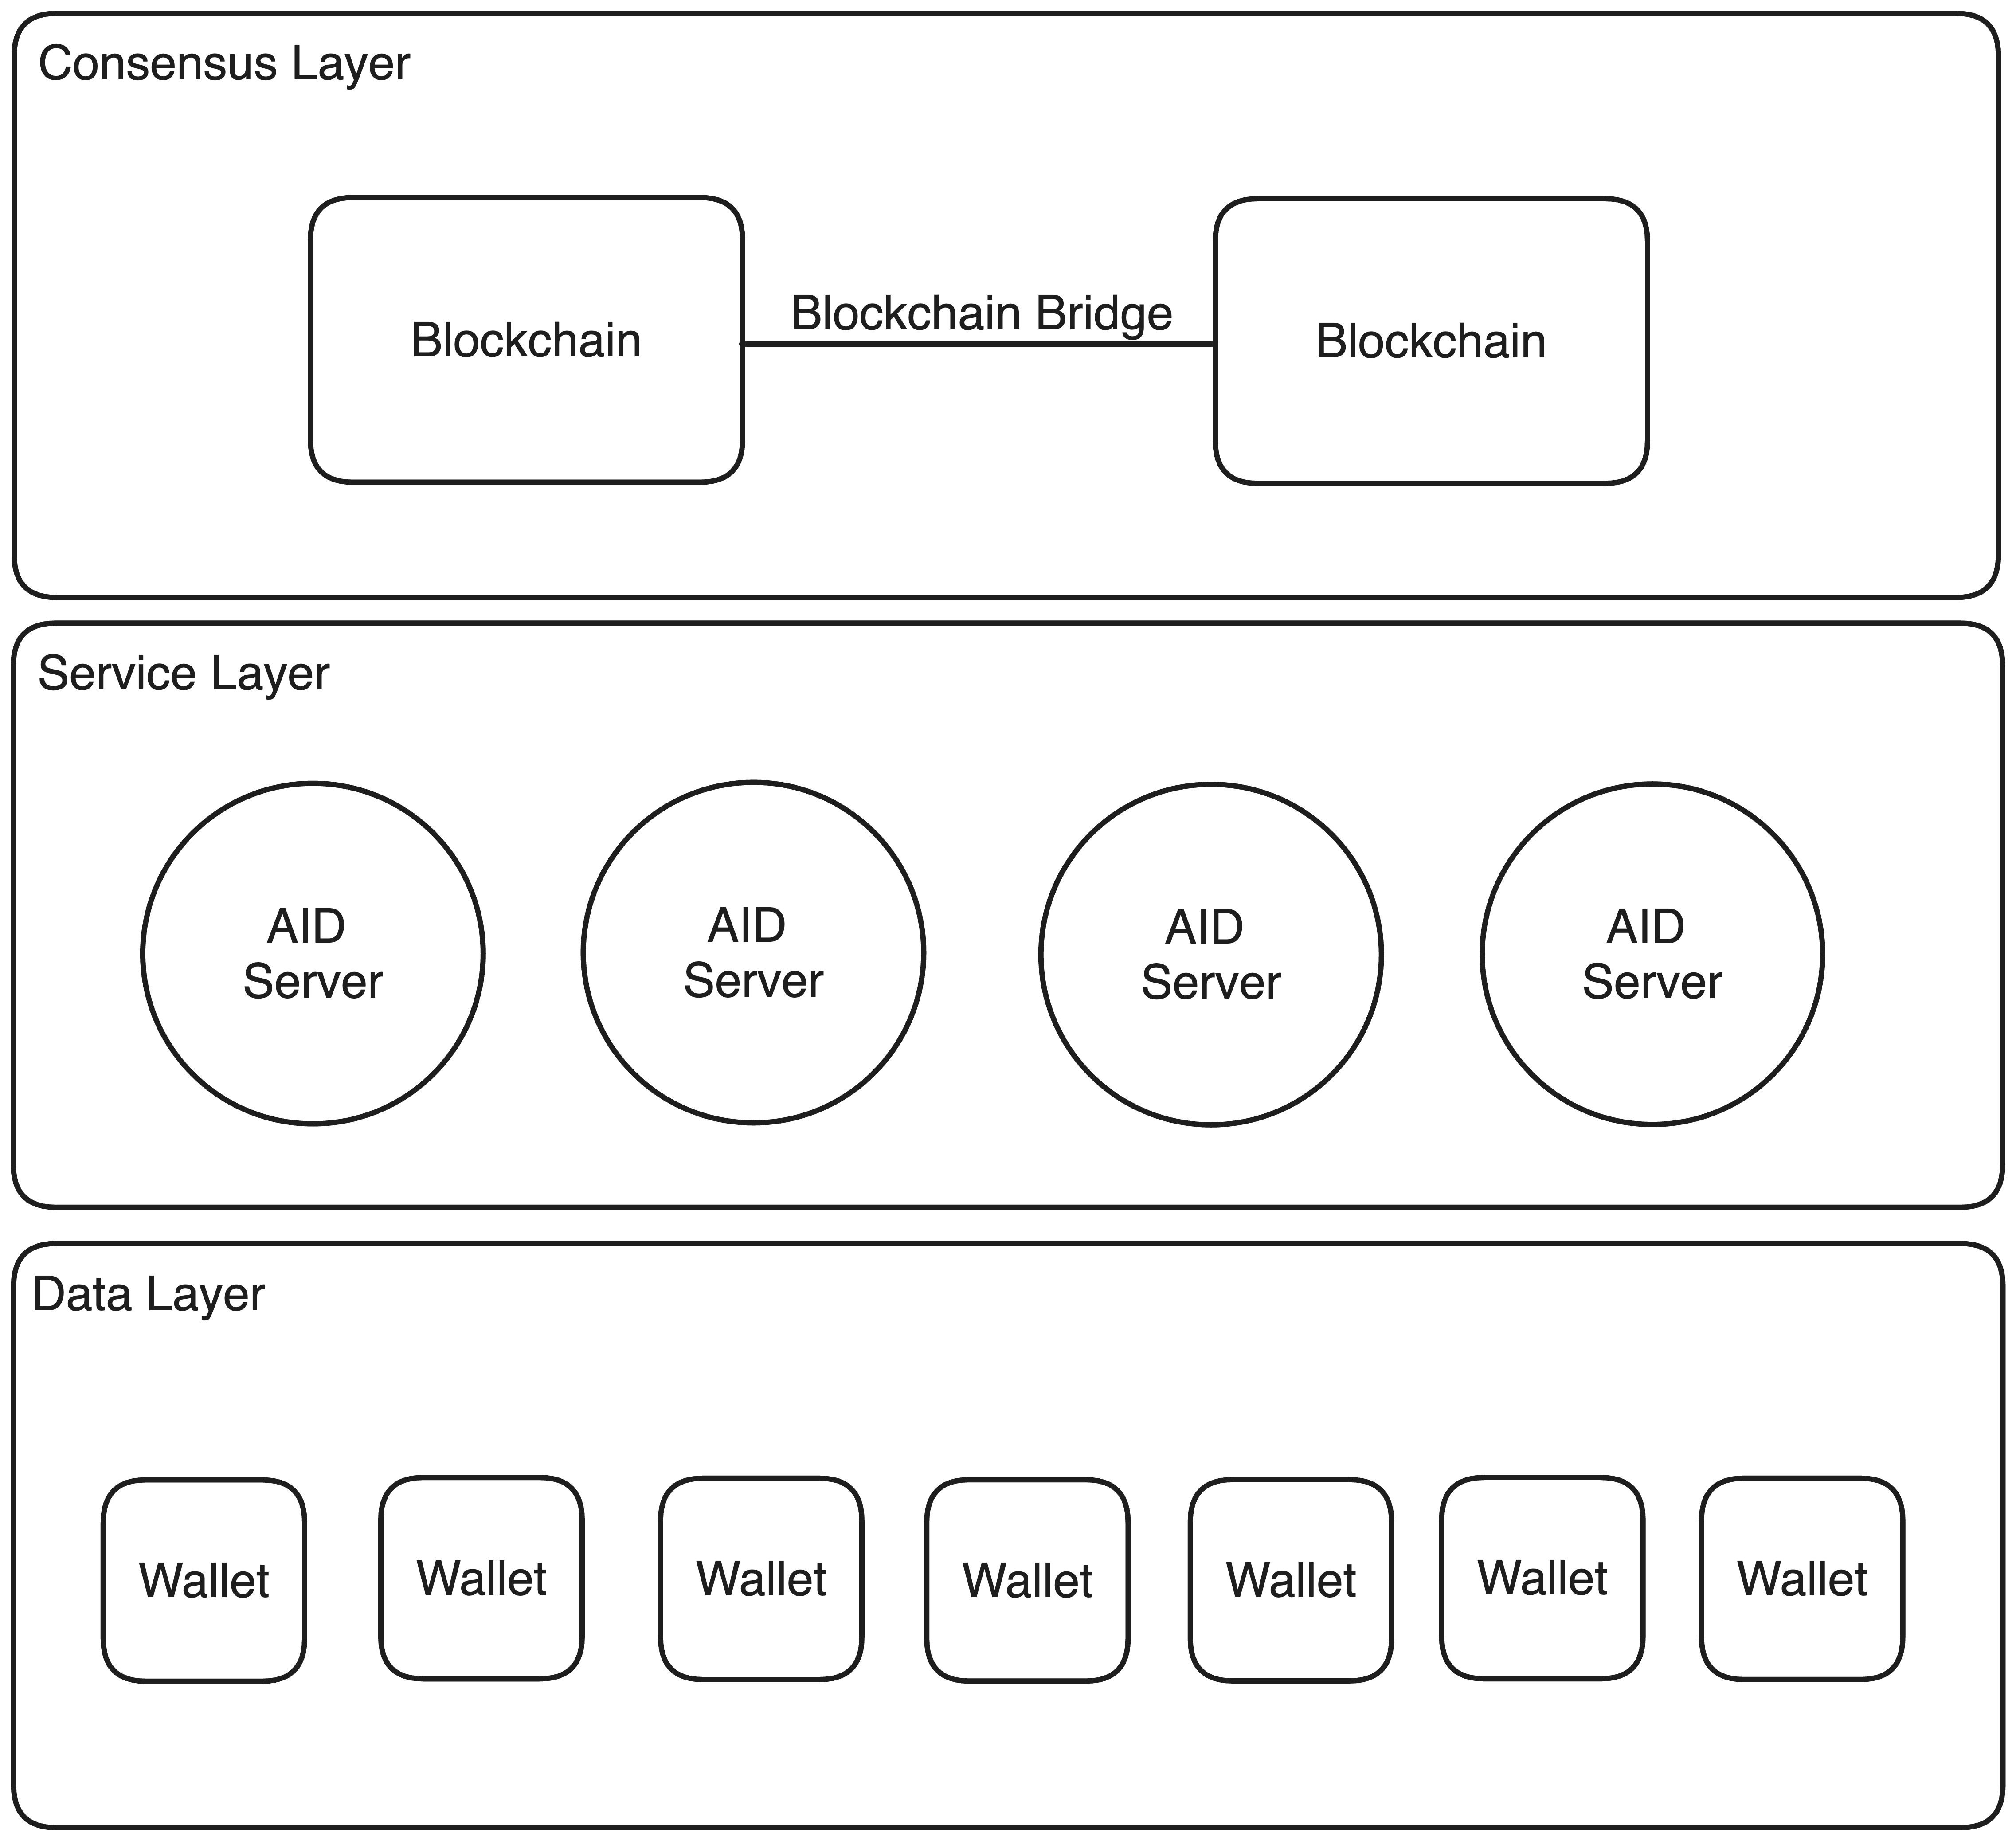
\includegraphics[width=0.8\textwidth]{figures/aidLayers.png}
  \caption{自主身份系統分層架構}
  \label{fig:aid-layers}
\end{figure}

更深入地看,共識層的核心組成是具備共識機制的區塊鏈系統。這一層級可通過跨鏈橋等先進機制實現水平擴展,顯著提升系統的可擴展性。區塊鏈中的智能合約扮演著關鍵角色,它為服務層和數據層提供了對共識數據進行讀寫操作的介面。值得注意的是,共識層的實現並不局限於區塊鏈技術。在存在可信第三方機構的情況下,其他形式的共識機制同樣可以被採用,這為系統設計提供了更大的靈活性。

服務層由多樣化且相互獨立的網路服務構成,這些服務可能以移動應用、網站或API服務等形式呈現。儘管各服務的具體需求可能大相徑庭,但它們都需要強大的身份管理功能。為了滿足這一普遍需求,我們提出了一個統一的解決方案:AID Server。我們設計了一個用於多種程式語言的後端SDK規格,它在保留客製化空間的條件下為服務提供者提供了一個標準化的身份管理介面。通過AID Server,服務開發者能夠輕鬆地實現與共識層和數據層的無縫對接,大大簡化了開發流程並維持了系統的一致性。

數據層主要由大量獨立的終端應用組成,這些應用可能是智能手機APP、個人電腦軟體或物聯網(IoT)設備等。與服務層類似,數據層中的應用雖然功能各異,但都需要可靠的身份管理能力。針對這一需求,我們設計了名為Wallet的前端SDK規格。Wallet能在多種程式語言下為應用開發者提供統一的身份管理介面。這使得開發者能夠輕鬆地實現數據層應用與共識層和服務層的有效對接,從而構建出一個完整且高效的生態系統。

這種多層架構設計不僅確保了系統各部分的模組化和解耦,還提高了整體系統的可擴展性、靈活性和安全性。通過標準化的介面和SDK規格,我們大大降低了開發難度,同時提高了不同層級間的互操作性。接著,我們將進一步介紹各層的的具體規格與設計細節。
\subsection{共識層}
共識層是自主身份系統的基礎建設,主要由無數個智能合約組成。並且,所有智能合約都應該包含以下四個功能,分別介紹:
\begin{itemize}
  \item \textbf{數據寫入:} 將特定格式的數據雜湊寫入區塊鏈,並提供即時的評價與狀態寫入功能。
  \item \textbf{數據讀取:} 讀取區塊鏈上特定數據的雜湊,並獲取相關評價與狀態資訊。
  \item \textbf{狀態更新:} 由證書擁有者執行,用於即時變更證書狀態,如撤銷或停用。
  \item \textbf{評價機制:} 允許用戶根據智能合約規則,以特定格式留下評價內容。
\end{itemize}
為了更好地理解共識層的運作,讓我們以學歷驗證為例。在這個場景中,用戶向學校申請學歷證明,學校將證明的數位簽名寫入區塊鏈。任何需要驗證該學歷的服務都可以通過讀取區塊鏈上的簽名來確認其真實性。若用戶的學歷狀態發生變化,學校可以即時更新區塊鏈上的簽名狀態,確保驗證方獲得最新資訊。此外,如果某企業對學歷證明的可信度存疑,可以在區塊鏈上留下評價,供其他驗證方參考。

為了保障用戶自主權,區塊鏈上寫入的簽名應遵循特定協議的智能合約,使用戶能自由決定操作簽名的規則。例如,用戶可以選擇具有刪除評價功能的智能合約來承載學歷證明的簽名,從而可以刪除特定的惡意評價。這種機制不僅保障了學歷資訊的即時性與真實性,還建立了一個動態且可自主控制的共識系統,大幅提升了身份管理系統的可靠性、效率及彈性。

然而,這樣的設計也面臨著諸多挑戰,首要問題是如何有效評價鏈上簽名,並將其轉化為影響用戶信譽的機制。其次,作為系統信任核心的區塊鏈,其長期穩定運營的可行性也是一個極需解決的問題。最後,在跨服務的用戶數據變化過程中,如何建立有效的共識機制同樣是一個關鍵議題。這些新架構下衍生的問題都需要深入探討和研究,以確保系統的可靠性和可持續性。

為了解決評價問題,我們必須理解為何在自主身份系統中,用戶需要在區塊鏈上的簽名留下評價。這涉及去中心化自治組織(DAO)的概念,我們可以將整個自主身份系統視為一個大型自治組織。在這個組織中,每個自主身份(AID)都是成員,每個成員都有信任和被信任的需求。傳統的中心化身份系統中,這種需求是由中心化的身份服務提供者來滿足的。而在自主身份系統中,這種需求則是通過區塊鏈上的評價來滿足。因此,我們可以將評價視為一種投票,其結果直接反映用戶的信譽。

值得注意的是,不僅用戶之間需要建立信任,用戶與服務之間也同樣需要。這種雙向信任的建立主要通過彼此評價來實現。因此,評價成為自主身份系統中的一個核心機制。評價機制的設計需要考慮諸多因素,如評價的權重、範圍和內容如何設定等。這些都涉及實際用戶的需求,我們希望保留用戶的自主權,讓他們可以自由選擇不同協議的智能合約作為區塊鏈上的評價機制。至於智能合約協議的協調與自治,我們期望能夠通過 DAO 中統治代幣的概念來實現。

作為系統信任核心的區塊鏈如何運營,這涉及到區塊鏈的經濟模型。我們提議在區塊鏈中發行一種逐漸增加的自主身份統治代幣。這種代幣可被抵押用於創建用戶的自主身份,藉此防止惡意用戶大規模創建惡意帳戶。每個自主身份(相當於其背後的代幣)可參與定期投票,討論評價機制的調整、新的智能合約協議等議題。為確保區塊鏈的長期運作,我們建議對失去信任的用戶實施懲罰,同時獎勵基礎設施的運作。因此,用於創建自主身份的代幣抵押後不可贖回,而是被鎖定在區塊鏈上。這樣可以確保用戶不會輕率創建自主身份,並激勵用戶維護自身自主身份的信譽。此外,我們建議對用戶在鏈上的每項操作採取使用者付費模式,使區塊鏈的維護者能獲得報酬,從而保證區塊鏈的持續運作。

最後,我們需要設計一個機制來實現跨服務的用戶數據變化共識。這是一個常見的網路服務需求,如微服務間的調用即為典型案例。在我們的設計中,資料的控制權從服務提供者轉移到用戶身上,這將大幅改變當前網路後端應用的設計。基於共識層的功能,我們提議讓用戶成為多個服務之間的橋樑。具體而言,用戶在區塊鏈外傳遞特定格式的資訊,而服務提供者則在區塊鏈上驗證這些資訊,從而達成共識。

舉例來說,在實作一個利用第三方支付服務的購票系統時,我們的方法與現行的網路後端設計有所不同。現有設計中,購票系統全權負責與支付體系的串接,用戶僅需與購票系統溝通。而在我們提出的架構下,流程如下:
\begin{enumerate}
  \item 購票系統要求用戶到銀行服務完成支付並取得收據。
  \item 銀行服務將收據的簽名寫入區塊鏈。
  \item 用戶向購票系統提交收據和購買請求。
  \item 購票系統在區塊鏈上驗證收據的真實性。
  \item 驗證通過後,完成購票流程。
\end{enumerate}
這種方式不僅確保了數據的可信度,還賦予了用戶更多對自身數據的控制權,體現了自主身份系統的核心理念。
\subsection{服務層}
服務層是自主身份系統的應用層,負責提供各種服務。自主身份系統不包含具體服務的實作,只是提供名為AID Server的後端SDK規格,讓服務開發者能夠輕鬆地把自己的應用接入自主身份系統。我們設計了AID Server的幾個關鍵功能:
\begin{itemize}
  \item \textbf{身份管理:} 提供服務註冊、登入、登出等基本身份管理功能。
  \item \textbf{證書管理:} 提供共識證書的創建、更新、讀取、評價等功能。
  \item \textbf{數據管理:} 提供用戶數據的導入、導出等功能。
\end{itemize}
以下將分別介紹這幾個功能的設計細節。
\subsubsection{身份管理}
對服務提供者而言,新的自主身份註冊必須提供基於「自主證書機制」創建的證書。此時,服務提供者可選擇是否接受該新自主身份。多數公開服務可能接受任何自主身份,但私人服務或有更高要求,如僅接受特定機構簽章的自主證書,或基於評價機制被充分信任的自主身份。一旦服務提供者接受新的自主身份,該身份即可開始使用服務。

自主身份系統的特點之一在於允許用戶自由標示自己的名稱,而非如傳統身份服務限制使用唯一的電子郵件地址作為用戶名。因此,提出了「別名優先機制」,使用戶可在註冊後自由選擇用戶名,無需擔心與他人重複。此設計不僅提高了用戶自主性,亦增加了隱私保護。

當用戶使用自主身份登入服務時,服務提供者要求按「自主證書」中預設的方法進行多因素驗證。例如,用戶可在自主證書中包含電子郵箱與手機號碼,服務提供者可要求用戶接收電子郵件驗證信或手機簡訊驗證碼。為避免使用者因驗證方式過於繁瑣而放棄使用服務,用戶可在登入後設置簡單的 PIN 碼,甚至允許在特定設備上免驗證登入。當用戶不再使用服務時,服務提供者應提供登出功能,清除簡易登入方案與狀態,以確保用戶資訊安全。

然而,此設計亦面臨諸多挑戰。首要問題是當用戶採用簡單方案登入時,可能因提供資訊不足而被攻擊者冒充或無法成功辨識身份。為此,我們提出「基於用戶時空的分析方法」作為系統性解決方案,通過追蹤用戶每次操作時夾帶或產生的資訊來辨識用戶身份,並配合「基於危險程度的驗證機制」找出應要求多因素驗證的時機。此設計在保留用戶便利性的同時,亦確保了安全性。

另一挑戰是如何在自主條件下,協助用戶處理忘記密碼的情況。自主身份應包含「極致多因素認證」概念,允許用戶在創建自主證書時設置多種驗證方案,包括難以遺失或忘記的方法,如生物特徵識別(指紋或臉部辨識)。如此,即使用戶忘記密碼,亦可通過這些驗證方式重新取回身份。進一步擴展此方案,我們可將「極致多因素認證」概念應用於「基於危險程度的驗證機制」,根據危險程度要求用戶使用多種方法完成多因素驗證,進一步提高安全性。
\subsubsection{證書管理}
證書管理在自主身份系統中扮演著雙重角色:一方面對用戶自主身份的證書進行操作,另一方面為實現「數據共識」機制而對證書進行操作。系統可通過讀取區塊鏈上用戶身份證書的狀態與簽名來完成驗證。此外,其他實體(如服務提供者或其他用戶)可基於自身經歷,在用戶證書對應的鏈上合約中留下評價。這樣的設計不僅有助於用戶在不同服務間建立信任,還能讓服務提供者更全面地了解用戶的信譽狀況。

在「數據共識」方面,當用戶申請共享特定數據時,服務提供者可按照預定的智能合約協議創建證書,並將證書簽名發布到區塊鏈上。如果數據發生變動,服務提供者可即時更新證書狀態,確保用戶數據的即時性和真實性。當另一個服務收到用戶在區塊鏈外提交的完整證書後,除了可以通過區塊鏈上的簽名驗證證書的真實性外,還可以在區塊鏈上留下評價,為其餘服務提供者提供參考。
\subsubsection{數據管理}
數據管理在服務層相對簡單,因為自主身份系統的核心在於賦予用戶控制自身數據的權利。理論上,服務提供者的最低要求是確保用戶能夠:
\begin{enumerate}
  \item 將當次操作所需的數據導入服務中
  \item 在操作結束後將數據導回用戶端
\end{enumerate}
然而,這種簡單設計可能大幅降低用戶體驗。例如:
\begin{itemize}
  \item 若用戶每次操作都需要導入和導出數據,前文提到的「基於用戶時空的分析方法」將變得不可行,因系統無法追蹤用戶操作。
  \item 頻繁的大量數據導入導出會顯著增加操作延遲和網路成本。
\end{itemize}
因此,「混合數據管理」模式成為必然選擇,即部分數據由用戶保管,部分由服務提供者保管。這種設計在保護用戶隱私的同時,也確保了操作的便利性。
然而,「混合數據管理」模式仍面臨諸多需要服務提供者與用戶達成共識的問題,包括:
\begin{itemize}
  \item 哪些數據由用戶管理?
  \item 哪些數據由服務提供者管理?
  \item 服務提供者管理的數據保留時間?
  \item 數據的使用權限?
\end{itemize}
這些問題涉及對隱私和資安的權衡。為確保用戶自主權,我們建議:
\begin{enumerate}
  \item 採用逐步詢問的方式協助用戶設定所有簡化的資安措施或降低的隱私保護措施。
  \item 設置應從高到低、從嚴格到寬鬆平滑過渡,使用戶能根據自身需求調整安全性和隱私保護程度。
\end{enumerate}
這種方法能在保護用戶權益的同時,為服務提供者提供必要的數據支持,實現雙方利益的平衡。透過這種「混合數據管理」模式,我們可以在自主身份系統中實現數據的高效管理,同時保障用戶的數據主權。
\subsection{數據層}
數據層是自主身份系統的存儲層,負責存儲用戶個人數據。我們設計了名為Wallet的前端SDK規格,讓數據層應用開發者能夠輕鬆地把自己的應用接入自主身份系統。Wallet的幾個關鍵功能如下:
\begin{itemize}
  \item \textbf{身份管理:} 提供自主身份的註冊、驗證等功能。
  \item \textbf{數據管理:} 提供用戶數據的上傳、下載等功能。
  \item \textbf{證書管理:} 對共識簽名的更新、讀取、評價等功能。
  \item \textbf{數據存儲:} 儲存用戶的數據。
\end{itemize}
以下將分別介紹這幾個功能的設計細節。
\section{資料結構}
\subsection{AID Server}
\subsection{Wallet}
\subsection{Consensus Core}
\section{自主身份系統的威脅模型}
\section{本章小結}
系統如何解決所有缺點,並且保留所有優點。

% !TeX root = ../main.tex

\chapter{實驗結果與討論}

可以這樣citation \cite{isensee2021nnu}。再多citation一個 \cite{IEEE-1363}。
\section{實驗說明}

\subsection{實驗環境}

\subsection{評估標準}


\section{參數分析}

% \lipsum

\section{腫瘤分割結果}

% \lipsum

\subsection{結果展示}

\subsection{與現有方法之數據比較}


% !TeX root = ../main.tex

\chapter{結論與未來展望}
本研究深入探討了自主身分(AID)系統,這是一個旨在解決現有身分管理系統挑戰的創新解決方案。通過將「自主」的概念融入數位身分管理,AID系統致力於在保障道德標準的同時,賦予使用者對其身分信息和數據的完全控制權。研究過程中,我們不僅提出了理論框架,還進行了系統設計和概念驗證,為未來的實際應用奠定了基礎。

本研究的主要貢獻包括:提出了創新的自主身分概念、設計了自主的身分管理機制、實現了高度的安全性和隱私保護、優化了使用者體驗、確保了法規遵循,並通過概念驗證展示了系統的可行性。

儘管AID系統展現出巨大潛力,但作為一個新興的研究領域,仍面臨諸多挑戰:
\begin{enumerate}
    \item \textbf{艱鉅的推廣任務:} AID系統可以說是一個全新的身分管理系統,需要克服使用者習慣、技術標準、法律法規等多方面的障礙。未來需要進一步研究如何推廣 AID 系統,提高使用者接受度和市場競爭力。
    \item \textbf{更高的開發難度:} AID系統不但使用了區塊鏈等新技術,還引入了反轉數據層等新概念,這將對開發人員的技術水平提出更高的要求。未來需要進一步研究如何降低開發難度。
    \item \textbf{大規模應用與部署:} 目前,AID系統的概念驗證主要集中在AI聊天服務和支付系統等有限的場景。未來需要進一步研究如何將AID系統應用於更廣泛的領域,例如金融、醫療、政務等,並探討大規模部署的可行性和挑戰。
\end{enumerate}

展望未來,AID系統有望在多個領域帶來革命性變革。在金融領域,它可以實現跨機構的無縫身分認證,簡化開戶和貸款流程,並建立更透明、公平的個人信用評估系統。在醫療領域,AID系統可以幫助建立患者完全掌控的電子病歷系統,實現跨機構就醫的同時保護患者隱私。在政務服務方面,基於AID的電子身分證系統可以實現一站式政務服務,而安全透明的電子投票系統則有助於提高公民參與度。

自主身分系統代表了數位身分管理的未來,有望成為下一個數位時代的代表性技術。儘管面臨挑戰,但通過持續研究和外部合作,AID系統將展現更廣闊的應用前景。未來研究將聚焦於大規模實際應用、使用者推廣、與現有系統的融合,以及系統性能和安全性的優化。我們期望更多人參與AID系統的探索和實踐,共同推動這一技術的發展,為數位社會的進步做出貢獻。

% 參考文獻
% References
\refmatter
\bibliographystyle{abbrv}
\bibliography{back/references.bib}

% 附錄
% Appendices
% !TeX root = ../main.tex

\appendix{A}{實際操作介面}
本附錄展示了本研究概念實作的部分功能截圖。
\section{AID錢包}
\begin{figure}
  \centering
  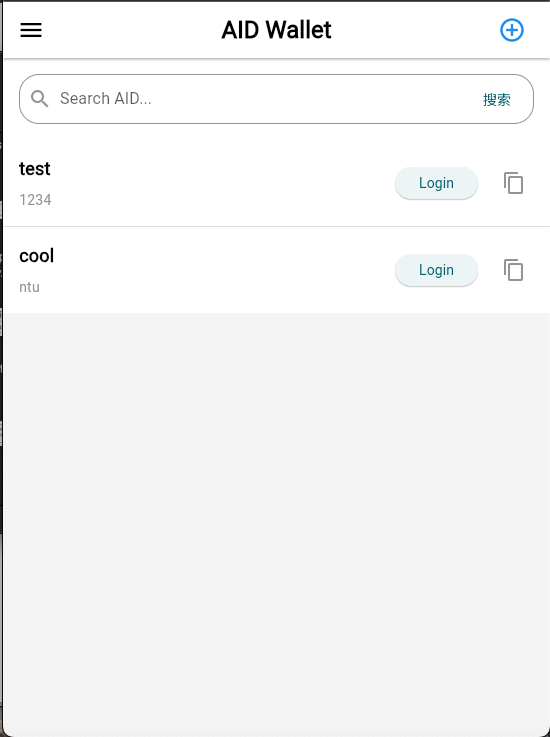
\includegraphics[width=\linewidth]{figures/wallet-demo.png}
  \caption{AID錢包}
  \label{fig:appendix-wallet}
\end{figure}
\clearpage
\begin{figure}[p]
  \centering
  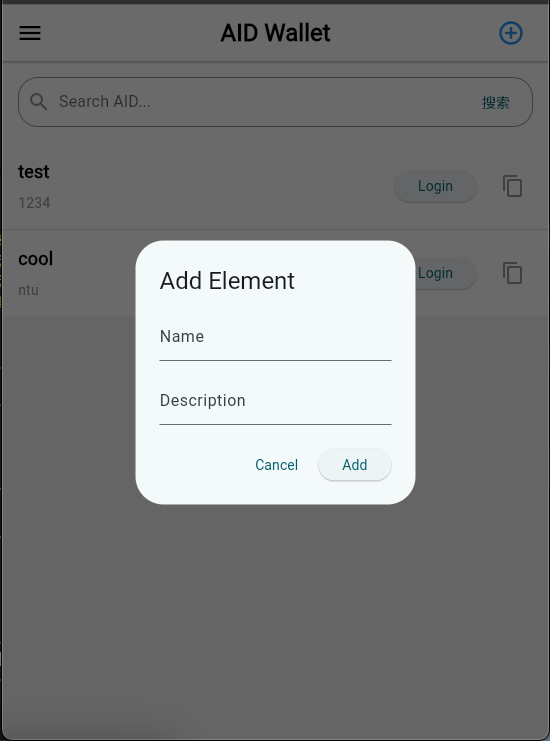
\includegraphics[width=\linewidth]{figures/wallet-create-demo.png}
  \caption{本地身份創建}
  \label{fig:appendix-wallet-create-demo}
\end{figure}
\clearpage
\begin{figure}[p]
  \centering
  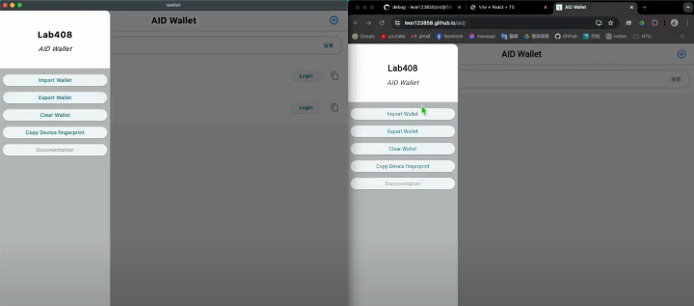
\includegraphics[width=\linewidth]{figures/wallet-drawer-demo.png}
  \caption{錢包遷移}
  \label{fig:appendix-wallet-drawer-demo}
\end{figure}
本節展示實作部分的AID錢包操作介面。
\begin{itemize}
  \item 圖\ref{fig:appendix-wallet}展示了AID錢包的實際操作介面。使用者可以通過錢包進行身分驗證、身份管理等操作。
  \item 圖\ref{fig:appendix-wallet-create-demo}展示了本地身份創建的操作流程。使用者可以通過錢包創建本地身份,並設置相關訊息。
  \item 圖\ref{fig:appendix-wallet-drawer-demo}展示了錢包遷移的操作流程。使用者可以通過錢包將本地身份遷移到其他設備上,實現身份的跨設備管理。
\end{itemize}
\section{AI聊天軟體}
\begin{figure}
  \centering
  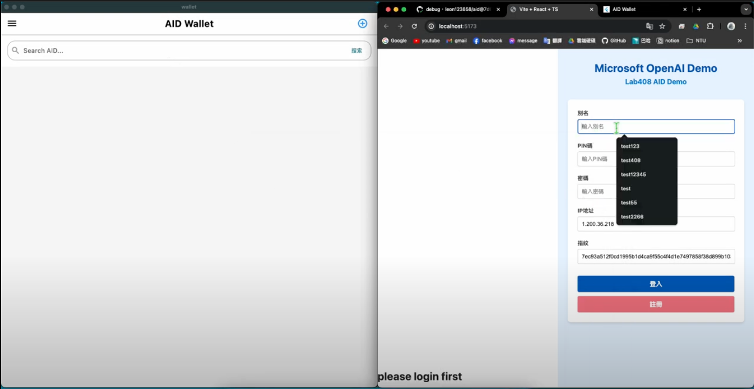
\includegraphics[width=\linewidth]{figures/AI-demo-logout.png}
  \caption{AI聊天軟體(未登入)}
  \label{fig:appendix-AI-demo-logout}
\end{figure}
\clearpage
\begin{figure}[p]
  \centering
  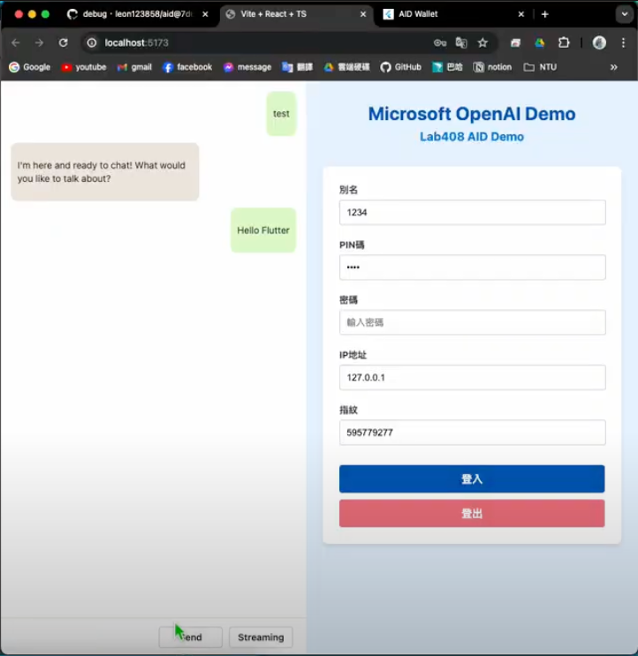
\includegraphics[width=\linewidth]{figures/AI-demo.png}
  \caption{AI聊天軟體(已登入)}
  \label{fig:appendix-AI-demo}
\end{figure}
本節展示實作部分的AI聊天軟體操作介面,使用者可以通過AID錢包登入並使用聊天功能。
\begin{itemize}
  \item 圖\ref{fig:appendix-AI-demo-logout}展示了AI聊天軟體的未登入狀態,使用者沒辦法使用聊天功能。
  \item 圖\ref{fig:appendix-AI-demo}展示了AI聊天軟體的已登入狀態,使用者可以通過AID錢包登入並直接聊天。
\end{itemize}

% !TeX root = ../main.tex

\appendix{B}{系統UML圖}
本附錄包含了自主身分(AID)系統的各種UML圖表,旨在從不同角度展示系統的結構、流程和交互。這些圖表有助於讀者更深入地理解AID系統的設計和運作機制。
\section{物件圖}
\begin{figure}
  \centering
  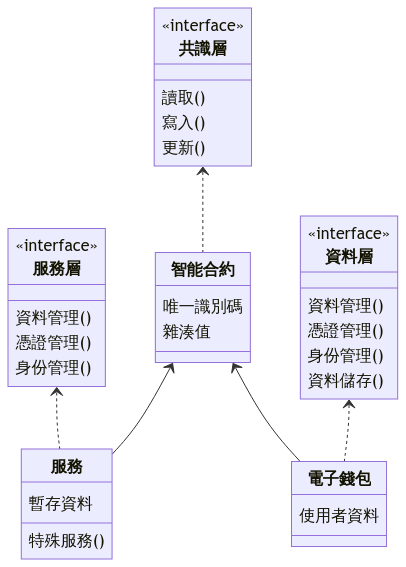
\includegraphics[width=\linewidth]{figures/design-struct.png}
  \caption{AID系統物件圖}
  \label{fig:appendix-aid-struct}
\end{figure}
物件圖展示了AID系統中各主要組件之間的靜態關係,有助於理解系統的整體架構。圖 \ref{fig:appendix-aid-struct} 呈現了AID系統的主要組件及其關係,包括共識層、服務層和數據層,以及它們之間的交互。
\section{時序圖}
時序圖展示了AID系統中各種重要流程的時間順序和組件間的交互,幫助讀者理解系統的動態行為。
\begin{itemize}
  \item 圖 \ref{fig:appendix-ca-uml} 展示了基本自主憑證的創建和使用流程,說明了用戶如何生成和管理自己的身份憑證。
  \item 圖 \ref{fig:appendix-da-uml} 描述了數據憑證的生成和驗證過程,展示了如何確保數據的真實性和可信度。
  \item 圖 \ref{fig:appendix-self-auth} 詳細說明了自主身分驗證的步驟,展示了用戶如何證明自己的身份。
  \item 圖 \ref{fig:appendix-full-aid-auth} 追加了第三方機構等額外功能的自主驗證流程,揭露更複雜場景的解決方案。
  \item 圖 \ref{fig:appendix-credit-uml} 展示了信用評分的計算和使用流程,說明了系統如何建立和維護用戶的信用。
\end{itemize}
\begin{figure}[p]
  \centering
  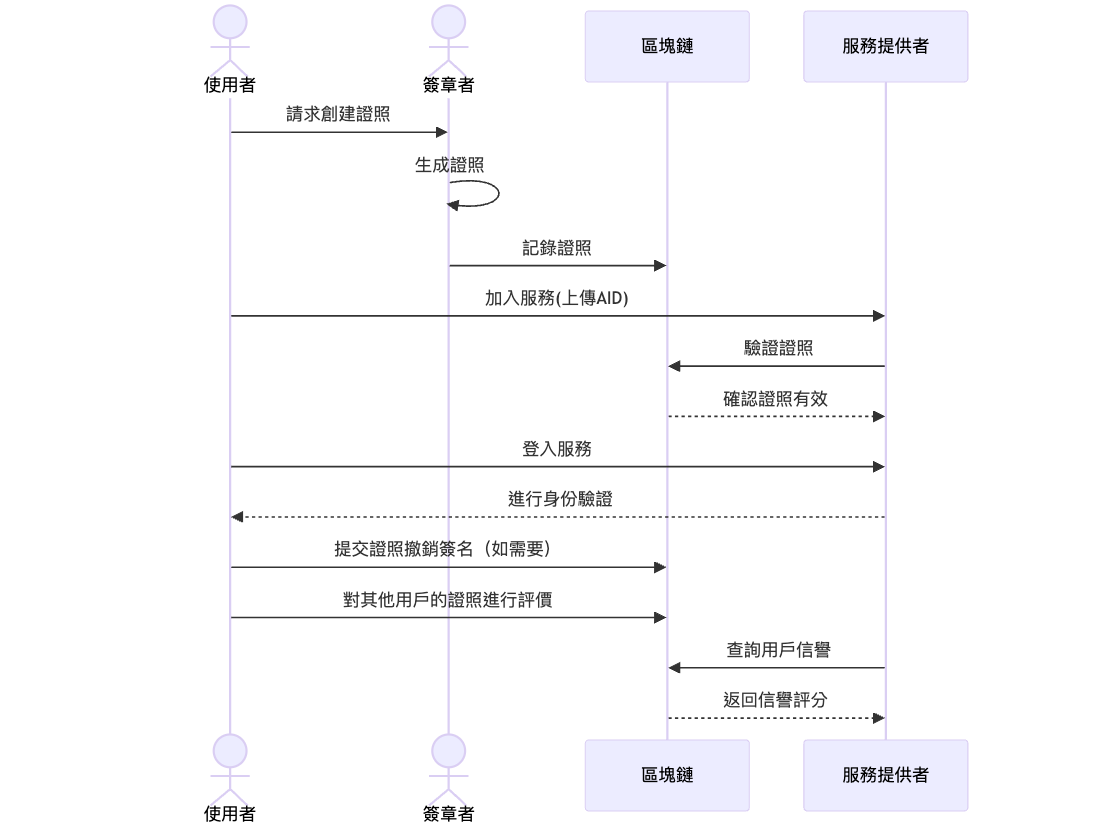
\includegraphics[width=\linewidth]{figures/CA-UML.png}
  \caption{自主憑證流程}
  \label{fig:appendix-ca-uml}
\end{figure}
\clearpage
\begin{figure}[p]
  \centering
  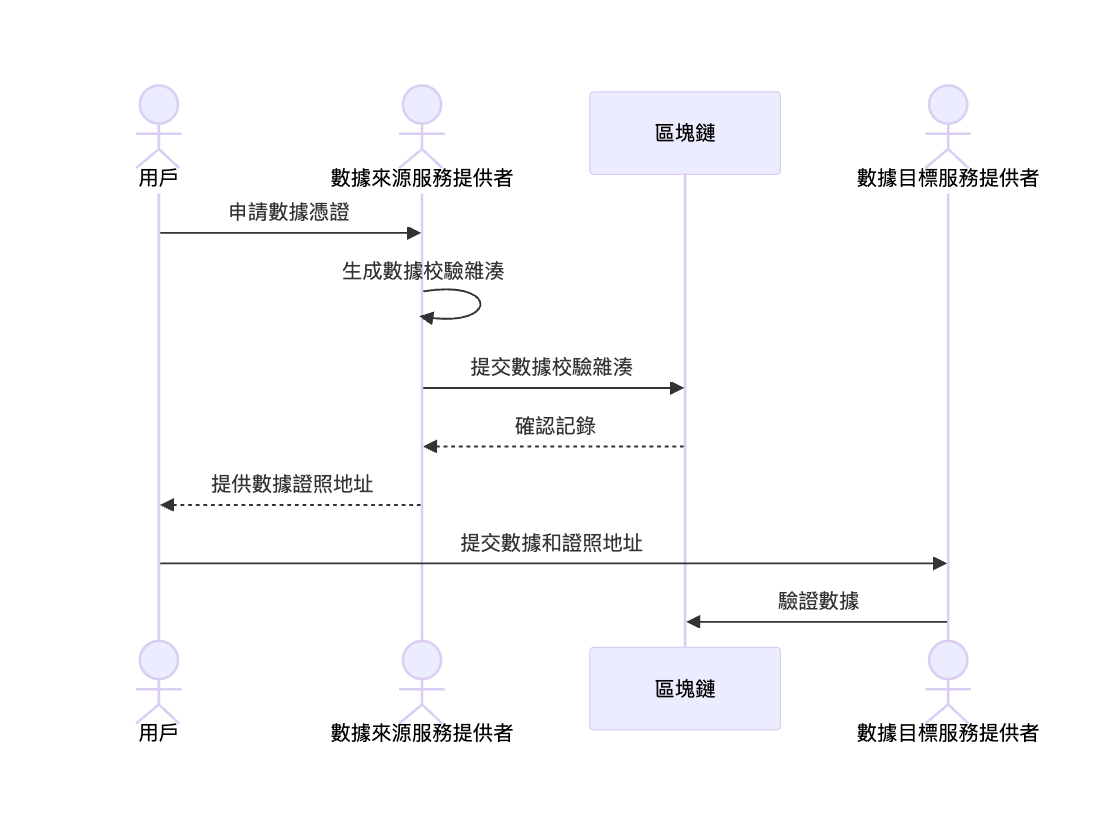
\includegraphics[width=\linewidth]{figures/DA-UML.png}
  \caption{數據憑證流程}
  \label{fig:appendix-da-uml}
\end{figure}
\clearpage
\begin{figure}[p]
  \centering
  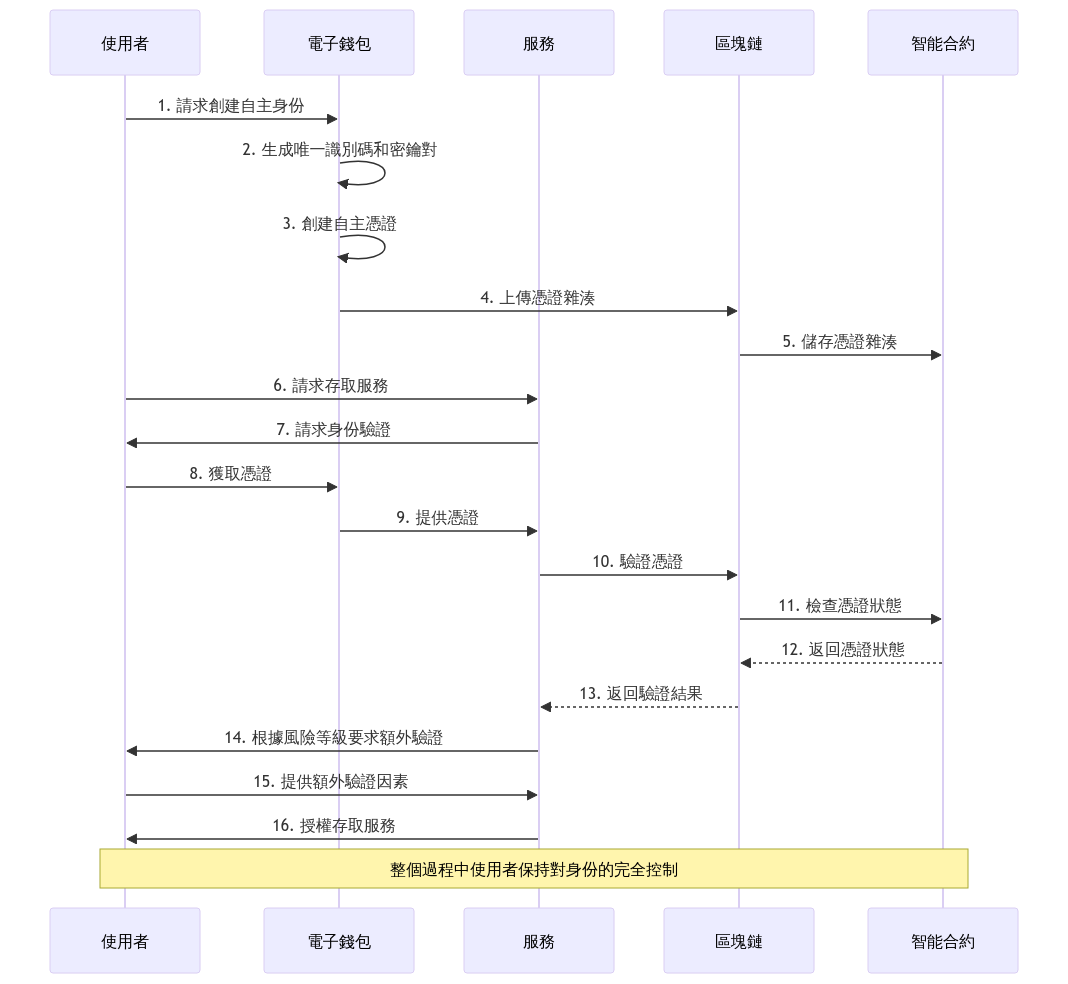
\includegraphics[width=\linewidth]{figures/new-self-auth.png}
  \caption{自主身分驗證流程}
  \label{fig:appendix-self-auth}
\end{figure}
\clearpage
\begin{figure}[p]
  \centering
  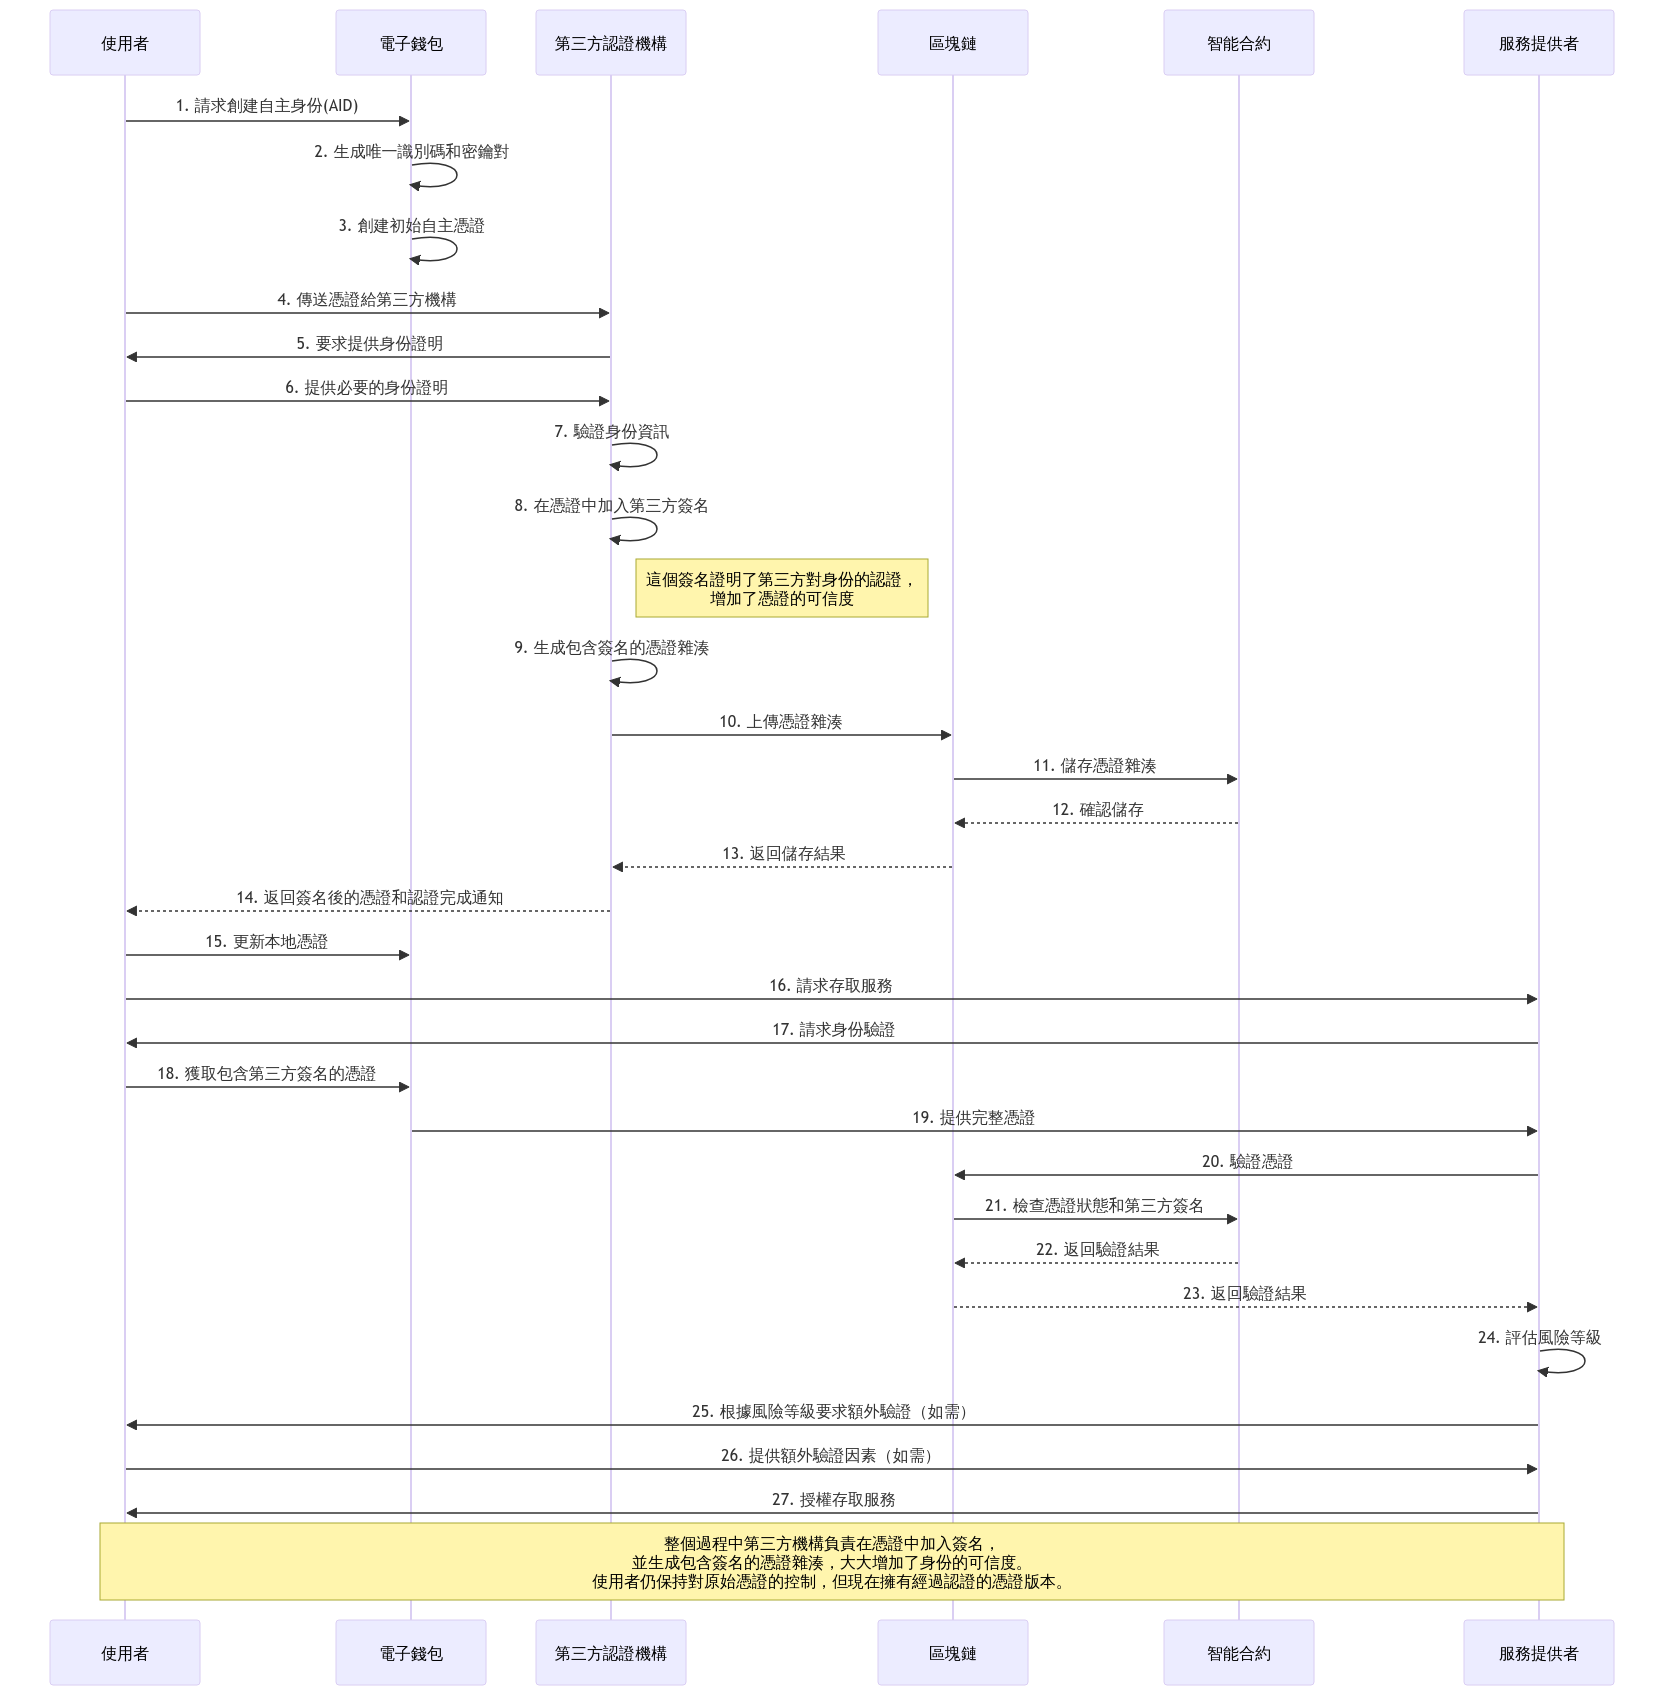
\includegraphics[width=\linewidth]{figures/full-aid-auth.png}
  \caption{AID系統完整自主驗證流程}
  \label{fig:appendix-full-aid-auth}
\end{figure}
\clearpage
\begin{figure}[p]
  \centering
  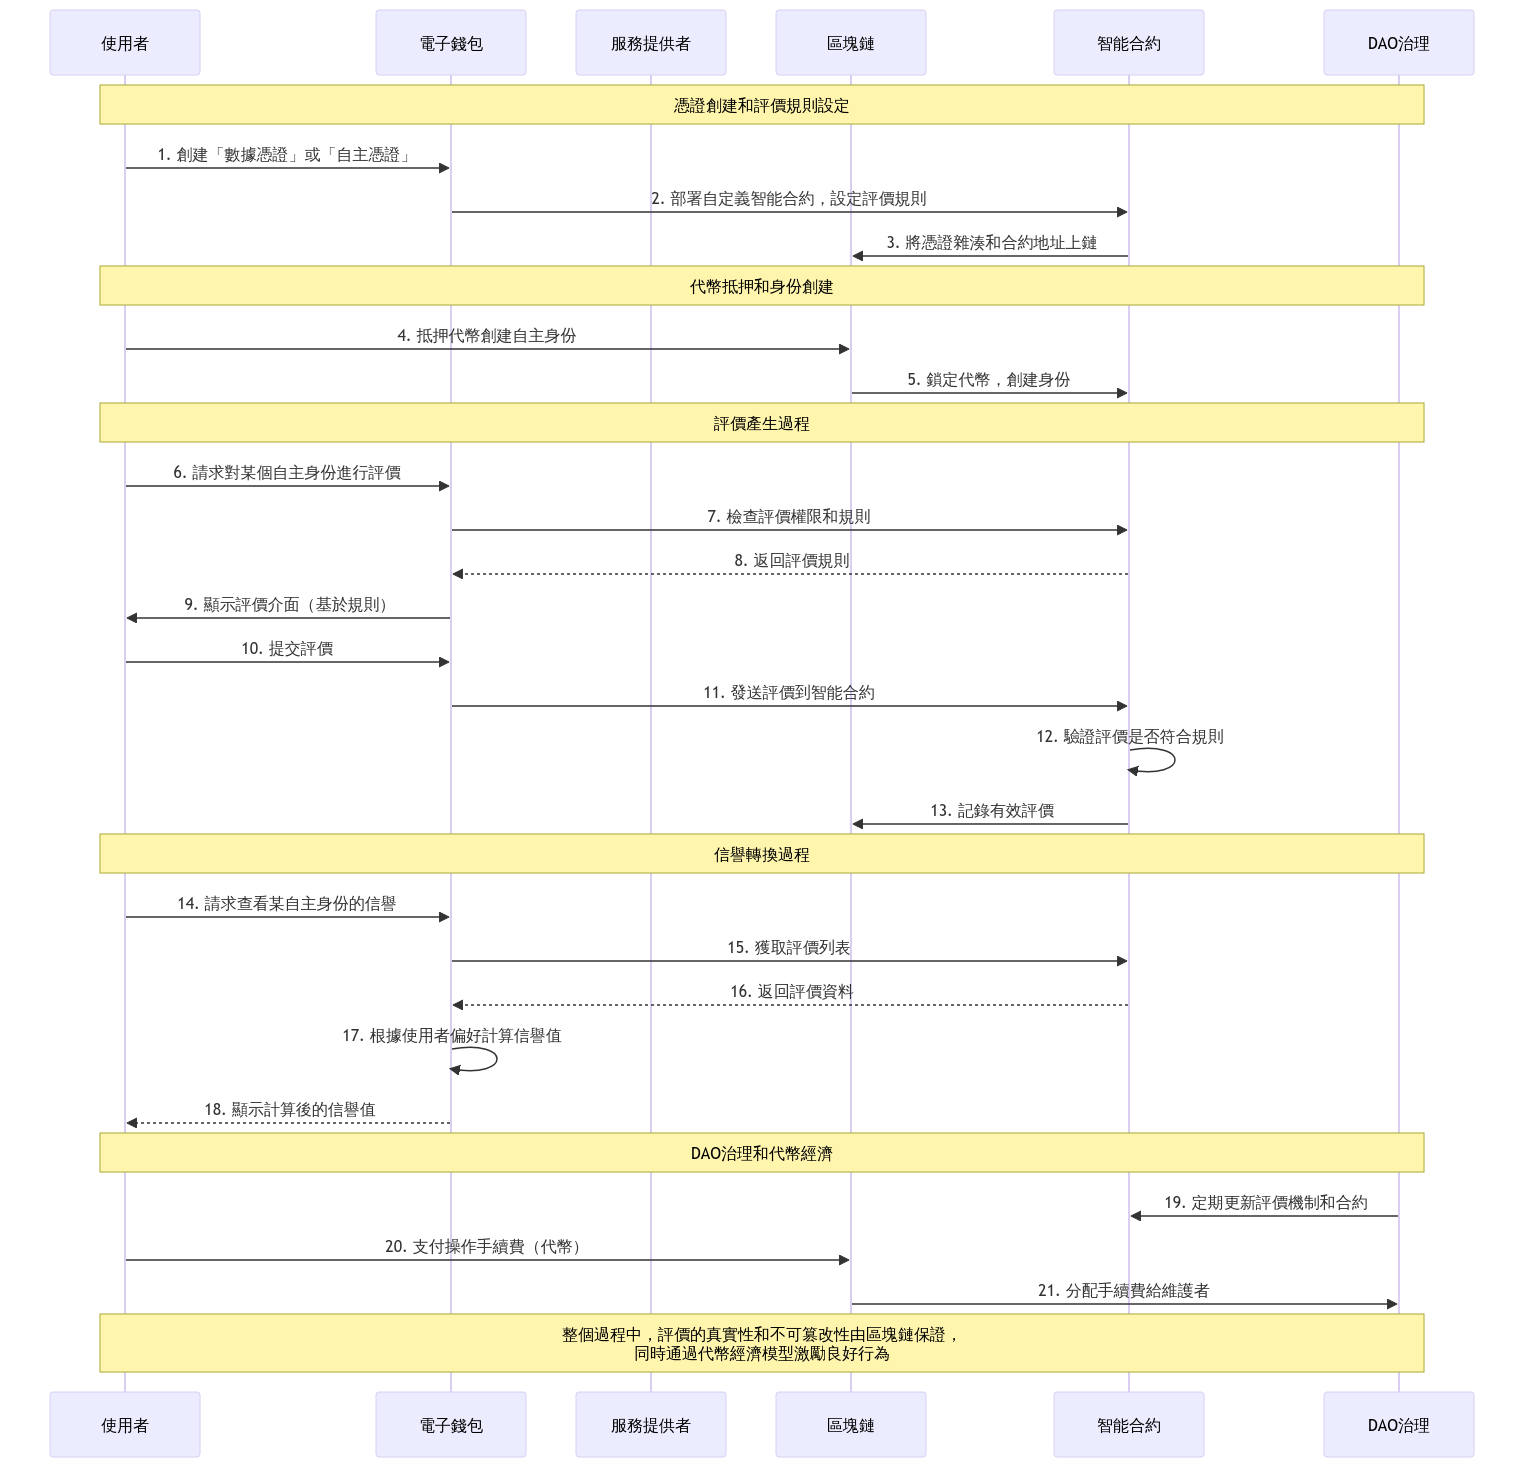
\includegraphics[width=\linewidth]{figures/credit-uml.png}
  \caption{信用評分流程}
  \label{fig:appendix-credit-uml}
\end{figure}
\section{流程圖}
流程圖詳細展示了AID系統中的特定流程,如多因素驗證和基於時空的分析,有助於理解系統的決策邏輯和操作步驟。
\begin{itemize}
  \item 圖 \ref{fig:appendix-emfa} 描述了極限多因素驗證的流程,展示了系統如何根據不同的風險級別要求不同程度的身份驗證。
  \item 圖 \ref{fig:appendix-time-space-analysis} 展示了基於時空的分析流程,說明了系統如何利用用戶的時間和空間信息來增強身份驗證的準確性。
\end{itemize}
\begin{figure}[p]
  \centering
  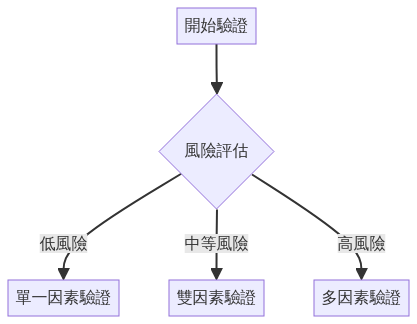
\includegraphics[width=0.5\linewidth]{figures/EMFA.png}
  \caption{極限多因素驗證流程}
  \label{fig:appendix-emfa}
\end{figure}
\clearpage
\begin{figure}[p]
  \centering
  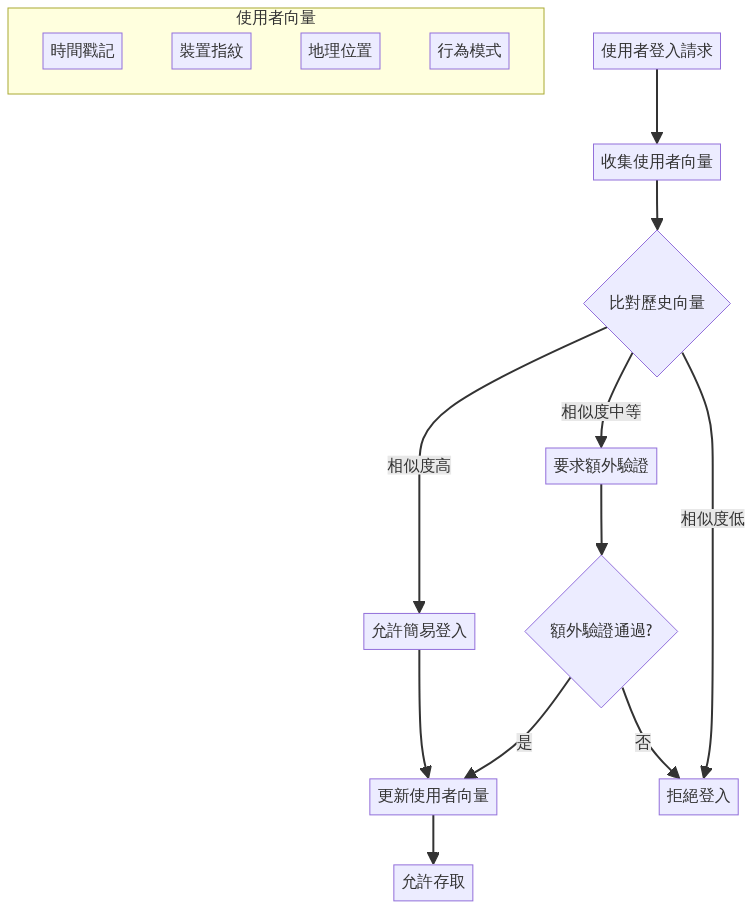
\includegraphics[width=\linewidth]{figures/time-space-analysis-uml.png}
  \caption{基於時空的分析流程}
  \label{fig:appendix-time-space-analysis}
\end{figure}

\end{document}
